\documentclass[a4paper]{article}
\usepackage[intlimits]{amsmath}
\usepackage{amssymb}
\usepackage{amsfonts}
\usepackage{listings}
\usepackage{courier}
\lstset{%
	basicstyle=\ttfamily,
	language=[LaTeX]tex, % Seems as if \lstset{language=tex} must be invoked BEFORE loading tikz!?
	tabsize=4,
	breaklines=true,
	breakindent=0pt
}

\usepackage{ifpdf}
\ifpdf
	\usepackage[pdftex]{hyperref}
	\pdfinfo {
		/Author	(Christian Feuersaenger)
	}

\else
	\usepackage[dvipdfm]{hyperref}
	\def\pgfsysdriver{pgfsys-dvipdfm.def}
\fi
%\def\pgfsysdriver{pgfsys-pdftex.def}
\usepackage{pgfplots}

\pgfrealjobname{pgfplotstest}

\def\testsection#1{\message{STARTING TEST SECTION '#1'}\section{#1}}
\def\testsubsection#1{\message{STARTING TEST SUBSECTION '#1'}\subsection{#1}}
\def\testsubsubsection#1{\message{STARTING TEST SUBSUBSECTION '#1'}\subsubsection{#1}}

\def\smallplotstest{%
\addplot[smooth,blue,mark=*] coordinates {
	(-1,	1)
	(-0.75,	0.5625)
	(-0.5,	0.25)
	(-0.25,	0.0625)
	(0,		0)
	(0.25,	0.0625)
	(0.5,	0.25)
	(0.75,	0.5625)
	(1,		1)
};
}

\def\loglogtestplot{
\addplot plot coordinates {
	(5,	8.311600e-02)
	(17,	2.546856e-02)
	(49,	7.407153e-03)
	(129,	2.101922e-03)
	(321,	5.873530e-04)
	(769,	1.622699e-04)
	(1793,	4.442489e-05)
	(4097,	1.207141e-05)
	(9217,	3.261015e-06)
};
\addlegendentry{$d=2$}

\addplot plot coordinates {
	(7,	8.471784e-02)
	(31,	3.044093e-02)
	(111,	1.022145e-02)
	(351,	3.303463e-03)
	(1023,	1.038865e-03)
	(2815,	3.196465e-04)
	(7423,	9.657898e-05)
	(18943,	2.873391e-05)
	(47103,	8.437499e-06)
};
\addlegendentry{$d=3$}
}%

\def\manylogplotsnolegend{%
	\addplot plot coordinates {
		(5,		8.312e-02)
		(17,	2.547e-02)
		(49,	7.407e-03)
		(129,	2.102e-03)
		(321,	5.874e-04)
		(769,	1.623e-04)
		(1793,	4.442e-05)
		(4097,	1.207e-05)
		(9217,	3.261e-06)
	};

	\addplot plot coordinates {
		(7,		8.472e-02)
		(31,	3.044e-02)
		(111,	1.022e-02)
		(351,	3.303e-03)
		(1023,	1.039e-03)
		(2815,	3.196e-04)
		(7423,	9.658e-05)
		(18943,	2.873e-05)
		(47103,	8.437e-06)
	};

	\addplot plot coordinates {
		(9,	7.881e-02)
		(49,	3.243e-02)
		(209,	1.232e-02)
		(769,	4.454e-03)
		(2561,	1.551e-03)
		(7937,	5.236e-04)
		(23297,	1.723e-04)
		(65537,	5.545e-05)
		(178177,	1.751e-05)
	};

	\addplot plot coordinates {
		(11,	6.887e-02)
		(71,	3.177e-02)
		(351,	1.341e-02)
		(1471,	5.334e-03)
		(5503,	2.027e-03)
		(18943,	7.415e-04)
		(61183,	2.628e-04)
		(187903,	9.063e-05)
		(553983,	3.053e-05)
	};

	\addplot plot coordinates {
		(13,	5.755e-02)
		(97,	2.925e-02)
		(545,	1.351e-02)
		(2561,	5.842e-03)
		(10625,	2.397e-03)
		(40193,	9.414e-04)
		(141569,	3.564e-04)
		(471041,	1.308e-04)
		(1496065,	4.670e-05)
	};
	\legend{$d=2$\\$d=3$\\$d=4$\\$d=5$\\$d=6$\\}
}%

\def\manylogplots{%
	\manylogplotsnolegend
	\legend{$d=2$\\$d=3$\\$d=4$\\$d=5$\\$d=6$\\}
}%

\author{Christian Feuers\"anger}
\title{Tests for pgfplots.sty}

\begin{document}
\maketitle
\tableofcontents

%--------------------------------------------------
\testfile{pgfplotstest.file.tex}
{%
\lstset{
	showtabs=true,
	showspaces=true,
	basicstyle=\footnotesize\ttfamily,
	numbers=left,
	numberblanklines=true,
	breaklines=false,
	tabsize=10}

\testsection{`plot file' test}
\testsubsection{A file in gnuplot format 'num num i'}
\lstinputlisting{plotdata/pgfplotstest_plot2.gnuplot}
\begin{tikzpicture}
\begin{axis}
\addplot plot file{plotdata/pgfplotstest_plot2.gnuplot};
\end{axis}
\end{tikzpicture}

\testsubsubsection{Same file loaded with `plot table'}
\begin{tikzpicture}
\begin{axis}
\addplot plot table{plotdata/pgfplotstest_plot2.gnuplot};
\end{axis}
\end{tikzpicture}


\testsubsection{A file which differs slightly from gnuplot format}
\lstinputlisting{plotdata/pgfplotstest_plot4}
\begin{tikzpicture}
\begin{axis}
\addplot plot file{plotdata/pgfplotstest_plot4};
\end{axis}
\end{tikzpicture}

\testsubsection{A file which starts with newlines}
\lstinputlisting{plotdata/pgfplotstest_plot5}
\begin{tikzpicture}
\begin{axis}
\addplot plot file{plotdata/pgfplotstest_plot5};
\end{axis}
\end{tikzpicture}

\testsubsubsection{Same file loaded with `plot table'}
The first data point should have been identified as column name.

\begin{tikzpicture}
\begin{axis}
\addplot plot table{plotdata/pgfplotstest_plot5};
\end{axis}
\end{tikzpicture}

\testsubsubsection{Same file loaded with `plot table from macro'}
{
\pgfplotstableread{plotdata/pgfplotstest_plot5}\TABLEMACRO
\begin{tikzpicture}
\begin{axis}
\addplot plot table from \TABLEMACRO;
\end{axis}
\end{tikzpicture}
}

\testsubsubsection{testing space gobbling in `plot file' command}
\begin{tikzpicture}
\begin{axis}
\addplot plot file {plotdata/pgfplotstest_plot2.gnuplot};
\end{axis}
\end{tikzpicture}

\testsubsubsection{testing plot file `skip first' option to skip header}
\begin{tikzpicture}
	\begin{loglogaxis}[title=Read from file `pgfplotstest\_plot']
	\addplot file[skip first] {plotdata/pgfplotstest_plot};
	\end{loglogaxis}
\end{tikzpicture}

\testsection{`plot table' test}
\begin{sidewaystable}
\lstinputlisting{plotdata/pgfplotstest_plot}
\caption{\texttt{pgfplotstest\_plot}}
\end{sidewaystable}
\testsubsection{Plot by column `dof' versus column `Lmax'}
\begin{tikzpicture}
\begin{loglogaxis}[xlabel=Dof,ylabel=$L_\infty$ error,title=Read from file `pgfplotstest\_plot']
\addplot plot table[x=dof,y=Lmax] {plotdata/pgfplotstest_plot};
\end{loglogaxis}
\end{tikzpicture}


\testsubsection{Inline Data Format}
\testsubsubsection{Defaults}
\begin{tikzpicture}
	\begin{axis}
		\addplot table {
			col1 col2
			1 1
			2 2
			3 3
			4 4
			5 5
			6 6
		};
	\end{axis}
\end{tikzpicture}

\testsubsubsection{with scanline detection + different input selectors}
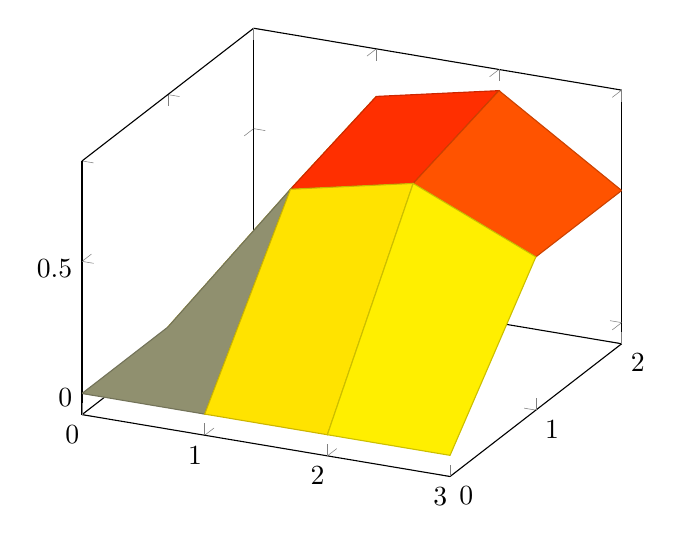
\begin{tikzpicture}
	\begin{axis}
		\addplot3[surf] table[y=col2,z expr=\thisrow{col3}*1] {
			col1 col2 col3
			 0 0 0
			 1 0 0
			 2 0 0
			 3 0 0 

			 0 1 0
			 1 1 0.6
			 2 1 0.7
			 3 1 0.5 

			 0 2 0
			 1 2 0.7
			 2 2 0.8
			 3 2 0.5 
		};
	\end{axis}
\end{tikzpicture}

\testsubsubsection{row sep=crcr}
\begin{tikzpicture}
	\begin{axis}
		\addplot table[row sep=crcr] {
			col1 col2\\
			1 1\\
			2 2\\
			3 3\\
			4 4\\
			5 5\\
			6 6\\
		};
	\end{axis}
\end{tikzpicture}

\testsubsubsection{row sep=crcr + macro arg}
{
	\def\content{
		\addplot table[row sep=crcr] {
			col1 col2\\
			1 1\\
			2 2\\
			3 3\\
			4 4\\
			5 5\\
			6 6\\
		};
	}
	\begin{tikzpicture}
		\begin{axis}
			\content
		\end{axis}
	\end{tikzpicture}
}
\testsubsubsection{row sep=crcr and col sep=ampersand}
\begin{tikzpicture}
	\begin{axis}
		\addplot table[col sep=&,row sep=\\] {
			col1 &col2\\
			1 &1\\
			2 &2\\
			3 &3\\
			4 &4\\
			5 &5\\
			6 &6\\
		};
	\end{axis}
\end{tikzpicture}

\testsubsubsection{row sep=crcr and col sep=ampersand}
\pgfplotstabletypeset[string type,col sep=&,row sep=\\]{
	col1 &col2\\
	1 &$1+1$\\
	2 &2\\
	3 &$3\cdot 4$\\
	4 &4\\
	5 &5\\
	6 &6\\
}

\pgfplotstabletypeset[columns/col1/.style={sci},columns/col2/.style={string type},col sep=&,row sep=\\]{
	col1 &col2\\
	1 &$1+1$\\
	2 &2\\
	3 &$3\cdot 4$\\
	4 &4\\
	5 &5\\
	6 &6\\
}

\testsubsubsection{row sep=crcr and scanline detection + different input selectors}
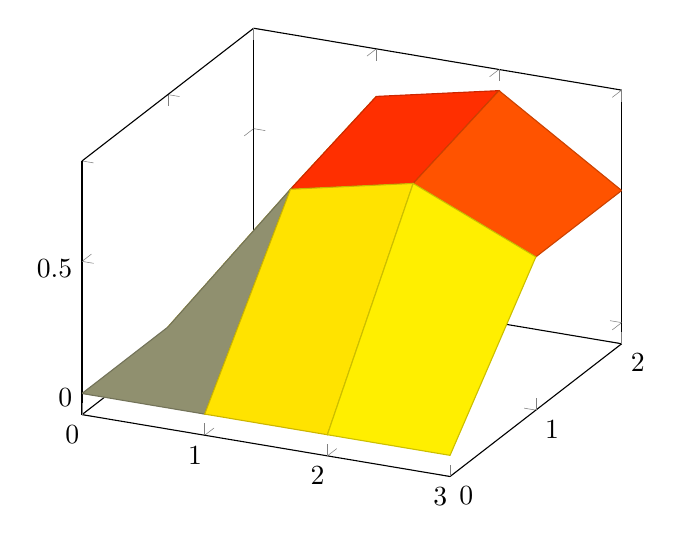
\begin{tikzpicture}
	\begin{axis}
		\addplot3[surf] table[y=col2,z expr=\thisrow{col3}*1,row sep=crcr] {
			col1 col2 col3\\
			 0 0 0\\
			 1 0 0\\
			 2 0 0\\
			 3 0 0 \\
\\
			 0 1 0\\
			 1 1 0.6\\
			 2 1 0.7\\
			 3 1 0.5 \\
\\
			 0 2 0\\
			 1 2 0.7\\
			 2 2 0.8\\
			 3 2 0.5 \\
		};
	\end{axis}
\end{tikzpicture}

{
\pgfplotstableset{
	alias/LmaxXX/.initial=Lmax,
	alias/{L/m=ax}/.initial=Lmax}
\testsubsection{Plot by column `dof' versus column `LmaxXX', a col alias}
\begin{tikzpicture}
\begin{loglogaxis}[xlabel=Dof,ylabel=$L_\infty$ error,title=Read from file `pgfplotstest\_plot']
\addplot plot table[x=dof,y=LmaxXX] {plotdata/pgfplotstest_plot};
\end{loglogaxis}
\end{tikzpicture}

\testsubsection{Plot by column `dof' versus column `L/m=ax', a col alias}
\begin{tikzpicture}
\begin{loglogaxis}[xlabel=Dof,ylabel=$L_\infty$ error,title=Read from file `pgfplotstest\_plot']
\addplot plot table[x=dof,y={L/m=ax}] {plotdata/pgfplotstest_plot};
\end{loglogaxis}
\end{tikzpicture}

\testsubsection{Plot by column `dof' versus column `L/m=ax', a col alias}
\begin{tikzpicture}
\begin{loglogaxis}[xlabel=Dof,ylabel=$L_\infty$ error,title=Read from file `pgfplotstest\_plot'; cdata using maxlevel]
\addplot+[scatter,point meta/expr=\thisrow{maxlevel}] plot table[x=dof,y={L/m=ax}] {plotdata/pgfplotstest_plot};
\end{loglogaxis}
\end{tikzpicture}

\testsubsection{Create on use}
\testsubsubsection{Typesetting the data with both, 'create on use' and col alias}
\pgfplotstabletypesetfile[
	create on use/order/.style={create col/dyadic refinement rate={L/m=ax}},
	columns={dof,L/m=ax,order},
]{plotdata/pgfplotstest_plot}

\testsubsubsection{Plotting data with col alias, scattersrc=ln(thisrow)}
\begin{tikzpicture}
	\begin{loglogaxis}[table/x=G,table/y={L/m=ax},]
	\addplot+[scatter,scatter src={ln(1e-8+\thisrow{L/m=ax})}] table {plotdata/pgfplotstest_plot};
	\end{loglogaxis}
\end{tikzpicture}

\testsubsubsection{Plotting data with 'create col/regression' feature}
\begin{tikzpicture}
\tracingmacros=2 \tracingcommands=2
	\begin{loglogaxis}[table/x=G,table/y={L/m=ax},]
	\addplot+[scatter,scatter src={ln(1e-8+\thisrow{L/m=ax})}] table {plotdata/pgfplotstest_plot};
	\addplot[red]
		table [y={create col/linear regression={y={L/m=ax},variance list={1000,1000,1000}}}]
		{plotdata/pgfplotstest_plot};
	\end{loglogaxis}
\end{tikzpicture}
}


\testsubsection{Plot by column \#2 versus column \#3}
\begin{tikzpicture}
\begin{loglogaxis}[
	xlabel=Dof,
	ylabel=$L_2$ error,
	title=Read from file `pgfplotstest\_plot'
]
\addplot plot table[x index=2,y index=3]{plotdata/pgfplotstest_plot};

\end{loglogaxis}
\end{tikzpicture}

\testsubsection{Plot by preloaded tables}
{
	\begin{sidewaystable}
		\lstinputlisting{plotdata/pgfplotstest_plot3}
		\caption{\texttt{pgfplotstest\_plot3}}
	\end{sidewaystable}
	\pgfnumtableread{plotdata/pgfplotstest_plot} to \tableA
	\pgfnumtableread{plotdata/pgfplotstest_plot3} to \tableB
	\begin{tikzpicture}
	\begin{loglogaxis}[
		xlabel=Dof,
		ylabel=$L_2$ error,
		title=Read from file `pgfplotstest\_plot' and `pgfplotstest\_plot3'
	]
		\addplot plot table[x=dof,y=L2] from \tableA;
		\addplot plot table[x=dof,y=L2] from \tableB;
		\legend{$d=2$\\$d=3$\\}%
	\end{loglogaxis}
	\end{tikzpicture}

	\testsubsubsection{Testing newline gobbling after optional args...}
	\pgfplotstabletypeset
		[sci,columns={dof,maxlevel}]
		\tableA

	\testsubsubsection{Testing newline gobbling in plot table}
	\begin{tikzpicture}
	\begin{loglogaxis}[
		xlabel=Dof,
		ylabel=$L_2$ error,
		title=Read from file `pgfplotstest\_plot'
	]
		\addplot table[x=dof,y=L2] 
			from 
			\tableA;
		\addplot table[x=dof,y=L2]
			{plotdata/pgfplotstest_plot};
		\legend{$d=2$\\$d=3$\\}%
	\end{loglogaxis}
	\end{tikzpicture}
}

\testsubsection{a table which has no column names}
\begin{sidewaystable}
\lstinputlisting{plotdata/pgfplotstest_plotnocolnames}
\caption{\texttt{plotdata/pgfplotstest\_plotnocolnames}}
\end{sidewaystable}
\begin{tikzpicture}
\begin{loglogaxis}[
	xlabel=Dof,
	ylabel=$L_2$ error,
	title=Read from file `pgfplotstest\_plotnocolnames'
]
\addplot plot table[x index=2,y index=3]{plotdata/pgfplotstest_plotnocolnames};

\end{loglogaxis}
\end{tikzpicture}

\clearpage
\testsection{Table Column Separators}


\long\def\testcolsep#1{%
	\lstinputlisting{plotdata/pgfplotstest_#1.dat}
	\pgfplotstabletypeset[col sep=#1]{plotdata/pgfplotstest_#1.dat}

	\begin{tikzpicture}
	\begin{axis}[
		title={col sep=#1.},
	]
	\addplot table[x=x,y=y,col sep=#1]{plotdata/pgfplotstest_#1.dat};

	\end{axis}
	\end{tikzpicture}
}
\testcolsep{comma}

\testcolsep{semicolon}

\testcolsep{colon}

\testcolsep{ampersand}

\testcolsep{braces}

	\lstinputlisting{plotdata/pgfplotstest_tab.dat}
	\pgfplotstabletypeset[col sep=tab]{plotdata/pgfplotstest_tab.dat}

	\begin{tikzpicture}
	\begin{axis}[
		title={col sep=tab.},
	]
	\addplot table[x=a long x name,y=y,col sep=tab]{plotdata/pgfplotstest_tab.dat};

	\end{axis}
	\end{tikzpicture}

\testsubsection{the same with active characters}
{
	\catcode`\;=13
	\def\testcolsep#1{%
		\begin{tikzpicture}
		\begin{axis}[
			title={col sep=#1.},
		]
		\addplot table[x=x,y=y,col sep=#1]{plotdata/pgfplotstest_#1.dat};

		\end{axis}
		\end{tikzpicture}
	}
	\testcolsep{semicolon}

	\catcode`\:=13
	\testcolsep{colon}
}

\testsection{`plot file' sanity checking test}
\testsubsection{2d}
\begin{tikzpicture}
	\begin{axis}[title=The input file has just one column.]
	\addplot file {plotdata/pgfplotstest_sanity.dat};
	\end{axis}
\end{tikzpicture}

\testsubsection{2d + meta}
\begin{tikzpicture}
	\begin{axis}[title=The input file has just one column.]
	\addplot+[scatter] file {plotdata/pgfplotstest_sanity.dat};
	\end{axis}
\end{tikzpicture}

\testsubsection{3d}
\begin{tikzpicture}
	\begin{axis}[title=The input file has just one column.]
	\addplot3 file {plotdata/pgfplotstest_sanity.dat};
	\end{axis}
\end{tikzpicture}

\testsubsection{3d + meta}
\begin{tikzpicture}
	\begin{axis}[title=The input file has just one column.]
	\addplot3+[scatter] file {plotdata/pgfplotstest_sanity.dat};
	\end{axis}
\end{tikzpicture}
}

\testfile{pgfplotstest.function.tex}
\testsection{`plot function' test}
\testsubsection{sin(x)}
\begin{tikzpicture}
\begin{axis}
\addplot plot[id=gnuplot_sin,samples=50] function{sin(x)};
\end{axis}
\end{tikzpicture}

\testsubsection{exp(x)}
\testsubsubsection{linear}
\begin{tikzpicture}
\begin{axis}
\addplot plot[id=gnuplot_exp,samples=50,domain=-5:15] function{exp(x)};
\end{axis}
\end{tikzpicture}

\testsubsubsection{semilogy}
\begin{tikzpicture}
\begin{semilogyaxis}
\addplot plot[id=gnuplot_exp,samples=50,domain=-5:15] function{exp(x)};
\end{semilogyaxis}
\end{tikzpicture}


\testsection{Testing path commands inside of axis}
\testsubsection{log plot}
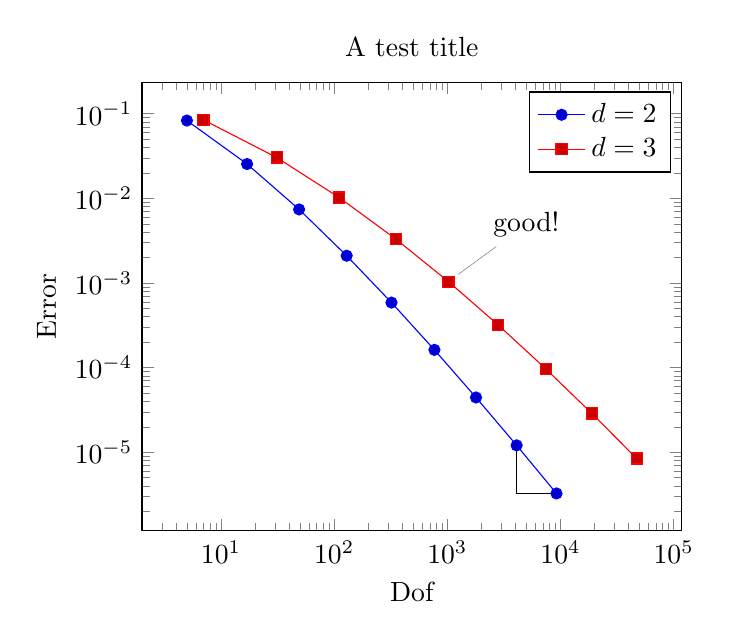
\begin{tikzpicture}
\begin{loglogaxis}[title=A test title,xlabel=Dof,ylabel=Error]
\loglogtestplot

\draw (axis cs:9217,	3.261015e-06) -| (axis cs:4097,	1.207141e-05);

\node[pin=45:good!] at (axis cs:1023,	1.038865e-03) {};
\end{loglogaxis}
\end{tikzpicture}

\testsubsection{Linear plot}
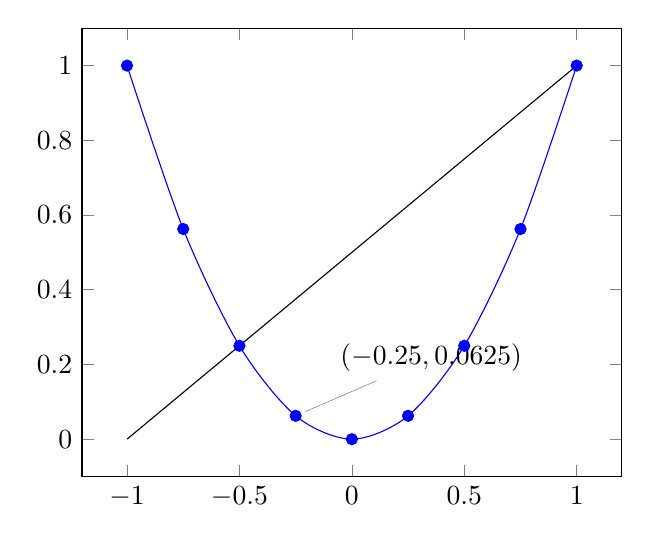
\begin{tikzpicture}
\begin{axis}
\smallplotstest

\draw (axis cs:-1,0) -- (axis cs:1,1);

\node[font=\footnotesize,pin=45:{$(-0.25,0.0625)$}] at (axis cs:-0.25,	0.0625) {};
\end{axis}
\end{tikzpicture}

\testsection{Checking plot expression}
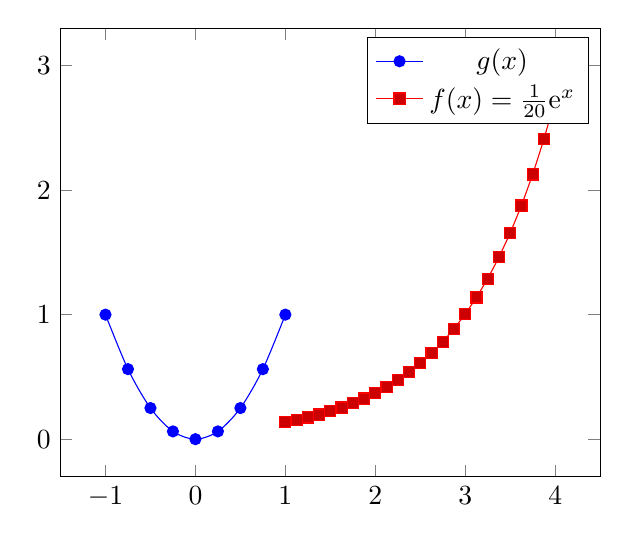
\begin{tikzpicture}
\begin{axis}[domain=1:4,ymin=0,ymax=3,enlargelimits]
\smallplotstest
\addlegendentry{$g(x)$}

\addplot (\x,{0.05*exp(\x)});
\addlegendentry{$f(x) = \frac{1}{20} \mathrm e^x$}
\end{axis}
\end{tikzpicture}
%
\testsection{Standard placement normal plot}
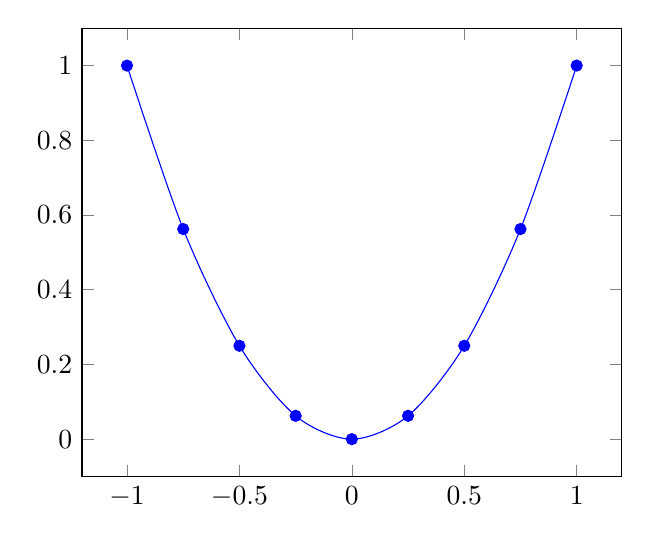
\begin{tikzpicture}
\begin{axis}
\smallplotstest
\end{axis}
\end{tikzpicture}


\testsection{Scaling tests}
\testsubsection{width=5cm}
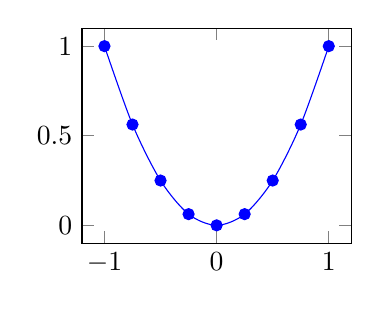
\begin{tikzpicture}
\begin{axis}[width=5cm]
\smallplotstest
\end{axis}
\end{tikzpicture}

\testsubsection{width=textwidth}
\begin{tikzpicture}
\begin{axis}[width=\textwidth]
\smallplotstest
\end{axis}
\end{tikzpicture}

\testsubsection{width=textwidth, height=textheight}
\begin{tikzpicture}
\begin{axis}[height=\textheight,width=\textwidth]
\smallplotstest
\end{axis}
\end{tikzpicture}

\testsubsection{height=3cm}
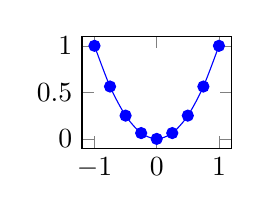
\begin{tikzpicture}
\begin{axis}[height=3cm]
\smallplotstest
\end{axis}
\end{tikzpicture}

\testsubsection{x=3cm}
\hrule width3cm height1pt
\vskip10pt
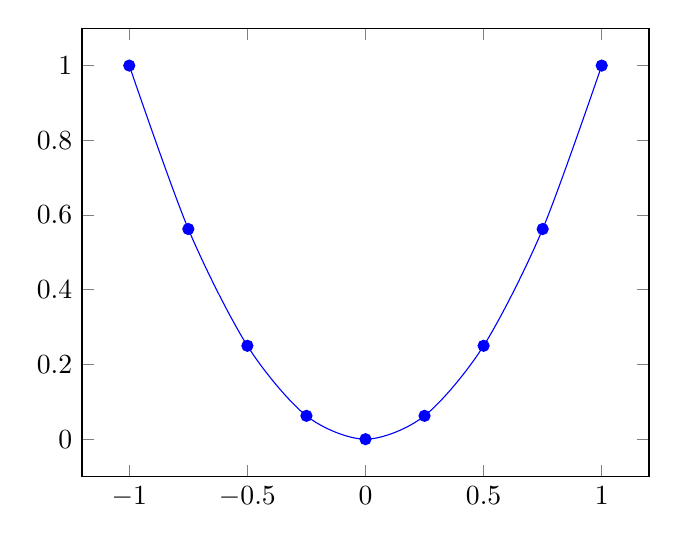
\begin{tikzpicture}[baseline]
\begin{axis}[x=3cm]
\smallplotstest
\end{axis}
\end{tikzpicture}

\testsubsection{x=3cm, y=4cm}
\hrule width3cm height1pt
\noindent
\vrule height4cm width1pt
\hskip10pt
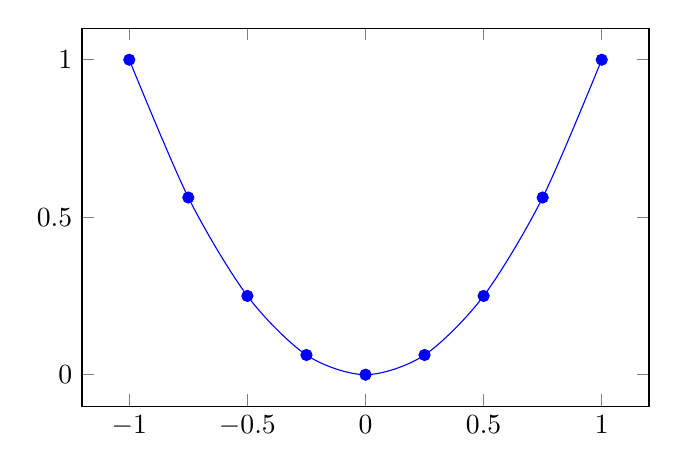
\begin{tikzpicture}[baseline]
\begin{axis}[x=3cm,y=4cm]
\smallplotstest
\end{axis}
\end{tikzpicture}

\testsubsection{y=3cm}
\noindent
\vrule height3cm width1pt
\hskip10pt
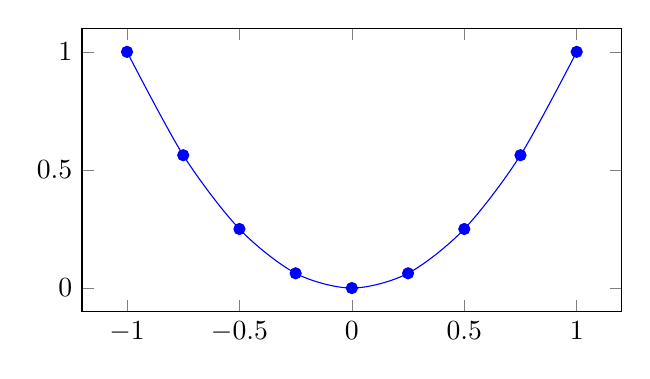
\begin{tikzpicture}[baseline]
\begin{axis}[y=3cm]
\smallplotstest
\end{axis}
\end{tikzpicture}

\testsubsection{Scale vs. Datascale trafo}
All should have the same size; especially the same height.
This tests the data scale transformation and rounding inaccuracies during the computation of $x$~and~$y$ unit vectors,
\[ x = \frac{W}{T(\bar x) - T(\underline x)}. \]
The larger $x$, the higher the scaling accuracy. Large $x$ means small $T(\bar x) - T(\underline x)$ (relative to width~$W$). But this implies low accuracy for the input data! And nobody wants inaccurate plots.

The datascale transformation~$T$ is set up such that $O(W) = O(x)$, but I am not sure if I need to adjust some parameters. Some parameters lead to inaccurate~$x$ and~$y$ vectors, such that axis sizes are \emph{not} the same although $W$~and~$H$ (width and height) are the same.

\noindent
{\tikzstyle{every picture}+=[baseline]
\tikzstyle{every axis}+=[width=3cm,scale only axis,ytick=\empty,cycle list=blue]%
\def\TESTPLOTS{%
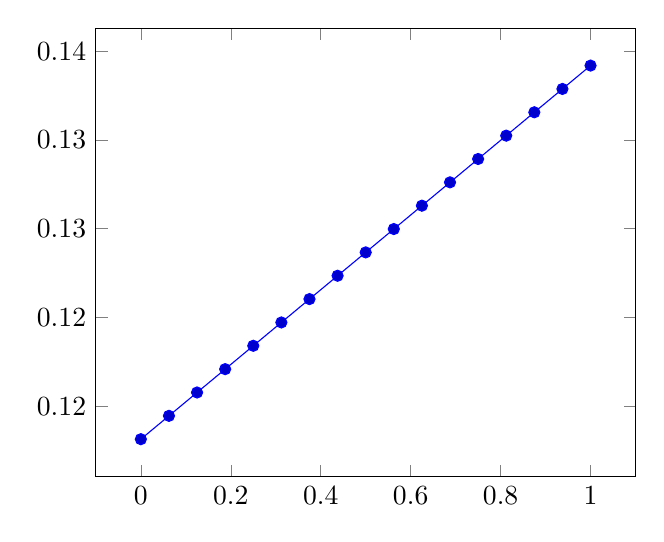
\begin{tikzpicture}%
\begin{axis}
\addplot plot coordinates {
	(0.000000,	0.113142)
	(0.062500,	0.114457)
	(0.125000,	0.115773)
	(0.187500,	0.117088)
	(0.250000,	0.118404)
	(0.312500,	0.119719)
	(0.375000,	0.121035)
	(0.437500,	0.122350)
	(0.500000,	0.123666)
	(0.562500,	0.124981)
	(0.625000,	0.126297)
	(0.687500,	0.127612)
	(0.750000,	0.128928)
	(0.812500,	0.130243)
	(0.875000,	0.131559)
	(0.937500,	0.132874)
	(1.000000,	0.134190)
};
\end{axis}
\end{tikzpicture}%
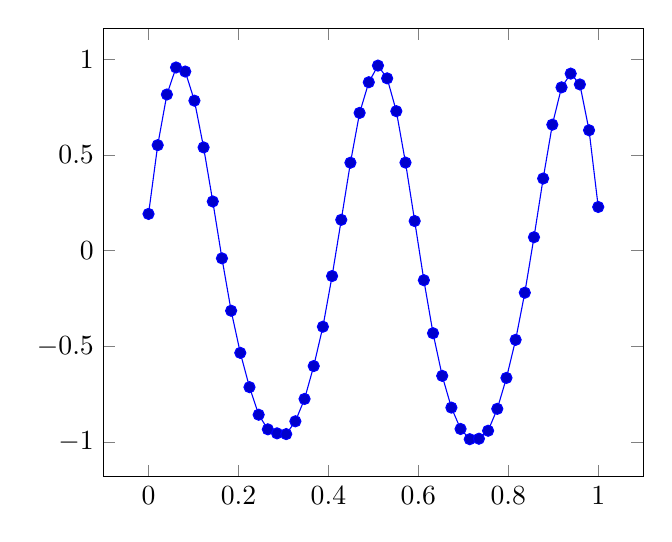
\begin{tikzpicture}%
\begin{axis}
\addplot plot coordinates {
	(0.000000,	0.192392)
	(0.020408,	0.551660)
	(0.040816,	0.816371)
	(0.061224,	0.957528)
	(0.081633,	0.936301)
	(0.102041,	0.784097)
	(0.122449,	0.539922)
	(0.142857,	0.257432)
	(0.163265,	-0.039651)
	(0.183673,	-0.313379)
	(0.204082,	-0.533386)
	(0.224490,	-0.712582)
	(0.244898,	-0.856655)
	(0.265306,	-0.932880)
	(0.285714,	-0.953862)
	(0.306122,	-0.957749)
	(0.326531,	-0.890993)
	(0.346939,	-0.774152)
	(0.367347,	-0.602360)
	(0.387755,	-0.396801)
	(0.408163,	-0.132261)
	(0.428571,	0.161664)
	(0.448980,	0.460018)
	(0.469388,	0.720198)
	(0.489796,	0.880398)
	(0.510204,	0.967384)
	(0.530612,	0.900632)
	(0.551020,	0.729232)
	(0.571429,	0.460479)
	(0.591837,	0.155311)
	(0.612245,	-0.153827)
	(0.632653,	-0.430787)
	(0.653061,	-0.653561)
	(0.673469,	-0.819444)
	(0.693878,	-0.931060)
	(0.714286,	-0.984394)
	(0.734694,	-0.981970)
	(0.755102,	-0.940272)
	(0.775510,	-0.825804)
	(0.795918,	-0.664138)
	(0.816327,	-0.465371)
	(0.836735,	-0.219185)
	(0.857143,	0.070697)
	(0.877551,	0.377456)
	(0.897959,	0.658660)
	(0.918367,	0.853564)
	(0.938776,	0.925472)
	(0.959184,	0.868936)
	(0.979592,	0.629528)
	(1.000000,	0.228732)
};
\end{axis}
\end{tikzpicture}%
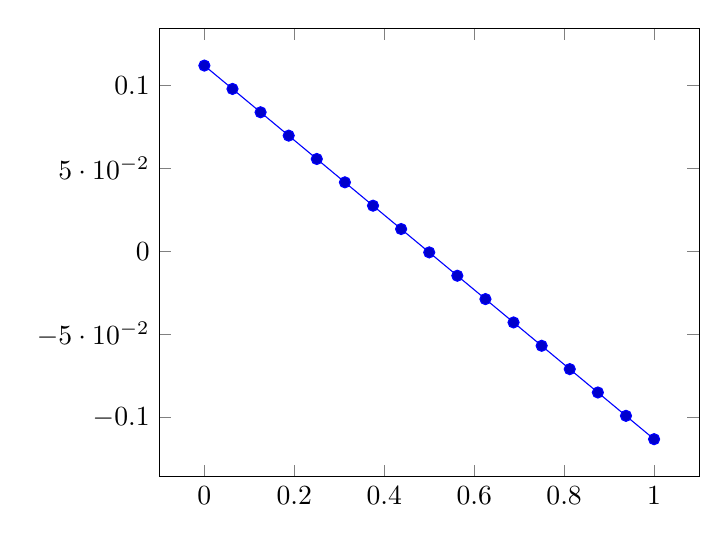
\begin{tikzpicture}%
\begin{axis}

\addplot plot coordinates {
	(0.000000,	0.112104)
	(0.062500,	0.098029)
	(0.125000,	0.083954)
	(0.187500,	0.069879)
	(0.250000,	0.055804)
	(0.312500,	0.041729)
	(0.375000,	0.027654)
	(0.437500,	0.013579)
	(0.500000,	-0.000496)
	(0.562500,	-0.014571)
	(0.625000,	-0.028646)
	(0.687500,	-0.042722)
	(0.750000,	-0.056797)
	(0.812500,	-0.070872)
	(0.875000,	-0.084947)
	(0.937500,	-0.099022)
	(1.000000,	-0.113097)
};
\end{axis}
\end{tikzpicture}%
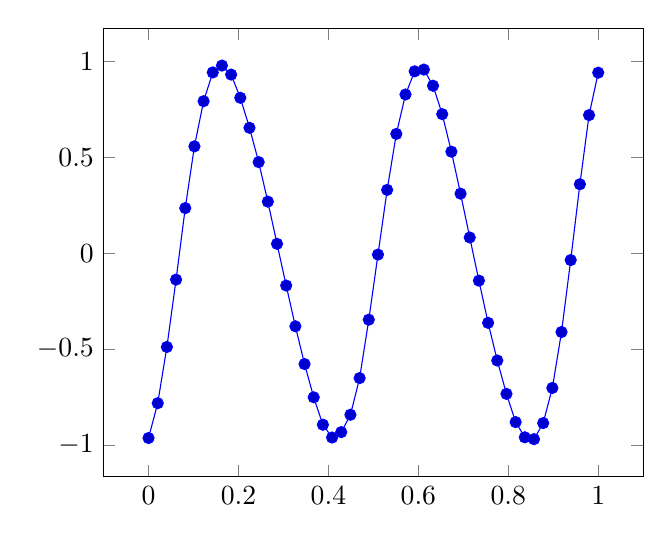
\begin{tikzpicture}%
\begin{axis}
\addplot plot coordinates {
	(0.000000,	-0.963159)
	(0.020408,	-0.781664)
	(0.040816,	-0.488585)
	(0.061224,	-0.137738)
	(0.081633,	0.234861)
	(0.102041,	0.556489)
	(0.122449,	0.791942)
	(0.142857,	0.941856)
	(0.163265,	0.977486)
	(0.183673,	0.930499)
	(0.204082,	0.809581)
	(0.224490,	0.653308)
	(0.244898,	0.474588)
	(0.265306,	0.268631)
	(0.285714,	0.048692)
	(0.306122,	-0.168568)
	(0.326531,	-0.380963)
	(0.346939,	-0.577633)
	(0.367347,	-0.751043)
	(0.387755,	-0.893755)
	(0.408163,	-0.960465)
	(0.428571,	-0.932380)
	(0.448980,	-0.841830)
	(0.469388,	-0.650880)
	(0.489796,	-0.346509)
	(0.510204,	-0.007265)
	(0.530612,	0.329744)
	(0.551020,	0.621489)
	(0.571429,	0.826905)
	(0.591837,	0.947602)
	(0.612245,	0.956706)
	(0.632653,	0.872426)
	(0.653061,	0.724325)
	(0.673469,	0.528915)
	(0.693878,	0.310032)
	(0.714286,	0.081807)
	(0.734694,	-0.143046)
	(0.755102,	-0.363063)
	(0.775510,	-0.559141)
	(0.795918,	-0.733031)
	(0.816327,	-0.880063)
	(0.836735,	-0.959350)
	(0.857143,	-0.968957)
	(0.877551,	-0.885145)
	(0.897959,	-0.702171)
	(0.918367,	-0.410704)
	(0.938776,	-0.035900)
	(0.959184,	0.359062)
	(0.979592,	0.719407)
	(1.000000,	0.940563)
};
\end{axis}
\end{tikzpicture}%
}%
\TESTPLOTS

once more again without `scale only axis':
\tikzstyle{every axis}+=[scale only axis=false]%

\TESTPLOTS
}

\testsubsection{Testing numeric artefacts around tick position `0'}
{\tikzstyle{every axis}+=[scaled ticks=false]
[scaled ticks=false] in this subsection

\begin{tikzpicture}
\begin{axis}
	\addplot coordinates {
		(-4.5,-8)
		(16,12)
	};
\end{axis}
\end{tikzpicture}

\begin{tikzpicture}
\begin{axis}
	\addplot coordinates {
		(-0.7,-8)
		(1.3,12)
	};
\end{axis}
\end{tikzpicture}

\begin{tikzpicture}
\begin{axis}
	\addplot coordinates {
		(-7000,-0.0008)
		(13000,0.0012)
	};
\end{axis}
\end{tikzpicture}
}

\testsection{Scaling log plots}
\hrule
\nobreak
\vskip10pt
\nobreak
\noindent
\begin{tikzpicture}
\begin{loglogaxis}[width=\textwidth]
\loglogtestplot
\end{loglogaxis}
\end{tikzpicture}

\begin{tikzpicture}
\begin{loglogaxis}[width=\textwidth,height=\textheight]
\loglogtestplot
\end{loglogaxis}
\end{tikzpicture}

\begin{tikzpicture}
\begin{loglogaxis}[height=5.5cm]
\loglogtestplot
\end{loglogaxis}
\end{tikzpicture}

\testsection{Scaletest}

{
\tikzstyle{every axis}+=[cycle list={%
	red,only marks,mark options={fill=red!80!black},mark=*\\%
	black,only marks,mark options={fill=black},mark=square*\\%
	}]
\begin{tikzpicture}
\begin{axis}[%
	width=8cm,
	height=2cm,
	xtick=\empty,
	ytick=\empty
]

\addplot plot coordinates {
	(0.968555,	0.000000)
	(0.984277,	0.000000)
	(0.030884,	0.000000)
	(0.250000,	0.000000)
	(0.750000,	0.000000)
	(0.468750,	0.000000)
	(0.750000,	0.000000)
	(0.484375,	0.000000)
	(0.968555,	0.000000)
	(0.968555,	0.000000)
	(1.000000,	0.000000)
	(1.000000,	0.000000)
	(0.030176,	0.000000)
	(0.250000,	0.000000)
	(0.250000,	0.000000)
	(0.250000,	0.000000)
	(0.750000,	0.000000)
	(1.000000,	0.000000)
	(0.500000,	0.000000)
	(0.500000,	0.000000)
	(0.234375,	0.000000)
	(0.500000,	0.000000)
	(0.750000,	0.000000)
	(0.000000,	0.000000)
	(0.750000,	0.000000)
	(0.468750,	0.000000)
	(0.500000,	0.000000)
	(0.000000,	0.000000)
	(0.468750,	0.000000)
	(0.000000,	0.000000)
	(0.750000,	0.000000)
	(0.000000,	0.000000)
	(0.234375,	0.000000)
	(1.000000,	0.000000)
};
\addplot plot coordinates {
	(0.367188,	0.000000)
	(0.625000,	0.000000)
	(0.312500,	0.000000)
	(0.656250,	0.000000)
	(0.312500,	0.000000)
	(0.148438,	0.000000)
	(0.125000,	0.000000)
	(0.640625,	0.000000)
	(0.136719,	0.000000)
	(0.875000,	0.000000)
	(0.390625,	0.000000)
	(0.828125,	0.000000)
	(0.875000,	0.000000)
	(0.656250,	0.000000)
	(0.125000,	0.000000)
	(0.343750,	0.000000)
	(0.861328,	0.000000)
	(0.312500,	0.000000)
	(0.578125,	0.000000)
	(0.578125,	0.000000)
	(0.625000,	0.000000)
	(0.375000,	0.000000)
	(0.875000,	0.000000)
	(0.812500,	0.000000)
	(0.847656,	0.000000)
	(0.589844,	0.000000)
	(0.343750,	0.000000)
	(0.125000,	0.000000)
	(0.875000,	0.000000)
	(0.125000,	0.000000)
	(0.609375,	0.000000)
	(0.156250,	0.000000)
};
\end{axis}
\end{tikzpicture}
}

\testsection{Scaling test for very small or very large x values}
{
\testsubsection{1e-2}
\begin{tikzpicture}
\begin{axis}
	\addplot plot coordinates {
		(0.005,1)
		(0.01,2)
		(0.02,4)
	};
\end{axis}
\end{tikzpicture}

\testsubsection{1e+2}
% \tracingmacros=2\tracingcommands=2
\begin{tikzpicture}
\begin{axis}
	\addplot plot coordinates {
		(50,1)
		(100,2)
		(200,4)
	};
\end{axis}
\end{tikzpicture}
% \tracingmacros=0\tracingcommands=0

\testsubsection{x=1e+11; y=1e-6}
{
%\tikzstyle{every x tick label}+=[font=\Huge]
%\tikzstyle{every x tick scale label}+=[anchor=base]
\begin{tikzpicture}
\begin{axis}
	\addplot plot coordinates {
		(5e10,1e-6)
		(1e11,2e-6)
		(2e11,4e-6)
	};
\end{axis}
\end{tikzpicture}
}

\testsubsection{1e+1}
\begin{tikzpicture}
\begin{axis}
	\addplot plot coordinates {
		(5,1)
		(10,2)
		(20,4)
	};
\end{axis}
\end{tikzpicture}

\testsubsection{1e+3}
\begin{tikzpicture}
\begin{axis}
	\addplot plot coordinates {
		(0.5,1e3)
		(10,2e3)
		(200,4e3)
	};
\end{axis}
\end{tikzpicture}

\testsubsection{1e+4}
\begin{tikzpicture}
\begin{axis}
	\addplot plot coordinates {
		(0.1,2e4)
		(0.2,4e4)
		(0.5,1e4)
	};
\end{axis}
\end{tikzpicture}

\testsubsection{1e-2, 1e+4}
\begin{tikzpicture}
\begin{axis}
	\addplot plot coordinates {
		(0.01,2e4)
		(0.02,4e4)
		(0.05,1e4)
	};
\end{axis}
\end{tikzpicture}
}

\testfile{pgfplotstest.ticks.tex}
\testsection{Minor ticks}

\begin{tikzpicture}
%\tracingmacros=2\tracingcommands=2
\begin{axis}[minor tick num=3]
\smallplotstest
\end{axis}
\end{tikzpicture}

\begin{tikzpicture}
\begin{axis}[minor tick num=1]
\smallplotstest
\end{axis}
\end{tikzpicture}

\begin{tikzpicture}
\begin{axis}[minor tick num=5]
\smallplotstest
\end{axis}
\end{tikzpicture}

\begin{tikzpicture}
%\tracingmacros=2\tracingcommands=2
\begin{axis}[minor tick num=5,xtick={0.5,1,2,2.5,3}]
\smallplotstest
\end{axis}
%\tracingmacros=0\tracingcommands=0
\end{tikzpicture}

\testsection{Tick placement}
\begin{tikzpicture}
\begin{axis}[
	xtick={-1.5,-1,...,1.5},
	ytick={-0.5,0,...,1.5},
	]
\smallplotstest
\end{axis}
\end{tikzpicture}

\begin{tikzpicture}
\begin{axis}[
	xmin=0,xmax=1,
	xtick={-1.5,-1.25,...,1.5}]
\smallplotstest
\end{axis}
\end{tikzpicture}

\testsubsection{xtick=data}
\begin{tikzpicture}
\begin{axis}[xtick=data,xmajorgrids]
\addplot coordinates {(0,0) (0.4,1) (1,2) (1.2,3) (4,5)};
\end{axis}
\end{tikzpicture}

\begin{tikzpicture}
\begin{axis}[xtick=data,xmajorgrids]
\addplot coordinates {(0,0) (0.4,1) (1,2) (1.2,3) (4,5)};
\addplot coordinates {(0.1,1) (0.5,2) (1.2,3)};
\end{axis}
\end{tikzpicture}

\begin{tikzpicture}
\begin{loglogaxis}[xtick=data,xmajorgrids]
\loglogtestplot
\end{loglogaxis}
\end{tikzpicture}

\testsubsubsection{ytick=data}
\begin{tikzpicture}
\begin{axis}[ytick=data,ymajorgrids]
\addplot coordinates {(0,0) (0.4,1) (1,2) (1.2,3) (4,5)};
\addplot coordinates {(0.1,1) (0.5,2) (1.2,3)};
\end{axis}
\end{tikzpicture}

\begin{tikzpicture}
\begin{loglogaxis}[ytick=data,ymajorgrids]
\loglogtestplot
\end{loglogaxis}
\end{tikzpicture}

\testsubsection{ticks on axis rectangle}
First plot: default tick style; second plot: red, third: 'help lines'

{\pgfplotsset{every axis/.append style={
	enlargelimits=false,
	xmin=-40,xmax=40,ymin=-40,ymax=40,
	xtick={-40,0,40},
	ytick={-40,0,40}
}}%
\begin{tikzpicture}
\begin{axis}[
]
\addplot coordinates {(-40,-40) (40,40)};
\end{axis}
\end{tikzpicture}
\begin{tikzpicture}
\begin{axis}[
	tick style={red,line width=5pt,major tick length=20pt},
]
\addplot coordinates {(-40,-40) (40,40)};
\end{axis}
\end{tikzpicture}
\begin{tikzpicture}
\begin{axis}[
	tick style={help lines},
]
\addplot coordinates {(-40,-40) (40,40)};
\end{axis}
\end{tikzpicture}
}

\testsubsection{modified labels}

{
\pgfplotsset{every axis label/.style={}}
\pgfplotsset{every axis x label/.style={
    at={(0.5,1)},
    above,
    yshift=+15pt}}
\pgfplotsset{every axis y label/.style={
    at={(1,0.5)},
    xshift=+35pt,
    rotate=90}}

\begin{tikzpicture}
\begin{axis}[
	xlabel=$x$ axis,
	ylabel=$y$ axis,
	xmin=0,xmax=1,
	tickpos=right,
	xtick={-1.5,-1.25,...,1.5}]
\smallplotstest
\end{axis}
\end{tikzpicture}
}

\begin{tikzpicture}
\begin{axis}[
	xlabel=$x$ axis,
	ylabel=$y$ axis,
	xmin=0,xmax=1,
	tickpos=both,
	xtick={-1.5,-1.25,...,1.5}]
\smallplotstest
\end{axis}
\end{tikzpicture}

\testsection{Tick label assigment tests}
\testsubsection{Using xticklabel and xtick}
\begin{tikzpicture}
\begin{axis}[
	xtick={-1.5,-1,...,1.5},
	xticklabel={%
		\ifcase\ticknum	$-1\frac12$%
		\or				$-1$%
		\or				$-\frac12$%
		\or				$0$%
		\or				$\frac12$%
		\or				$1$%
		\or				$1\frac12$%
		\else			$\tick$%
		\fi
	}
]
\smallplotstest
\end{axis}
\end{tikzpicture}

\testsubsection{Using xticklabels}%
\begin{tikzpicture}
\begin{axis}[
	xtick={-1.5,-1,...,1.5},
	xticklabels={%
		$-1\frac 12$,
		$-1$,
		$-\frac 12$,
		$0$,
		$\frac 12$,
		$1$}
]
\smallplotstest
\end{axis}
\end{tikzpicture}

\testsubsection{With xtick labels and commas by hand}
\begin{tikzpicture}
\begin{axis}[
	xtick={-1.5,-1,...,1.5},
	xticklabels={%
		{-1,5},
		-1,
		{-0,5},
		0,
		{0,5},
		1,
		{1,5}}
]
\smallplotstest
\end{axis}
\end{tikzpicture}

{
\testsubsection{Only with auto number formatting options; different for x and y}
%\tracingmacros=2\tracingcommands=2
\begin{tikzpicture}
\begin{axis}[
	xtick={-1.5,-1,...,1.5},
	x tick label style={/pgf/number format/use comma},
	y tick label style={/pgf/number format/.cd,use comma,fixed zerofill,precision=3},
]
\smallplotstest
\end{axis}
\end{tikzpicture}
}

\testsubsection{Using yticklabels in logplot}%
{
\def\tickformat#1{1e#1}%
\begin{tikzpicture}
\begin{loglogaxis}[
	ytick={1e-8,1e-7,1e-6,1e-5,1e-4,1e-3,1e-2,1e-1,1e0,1e1},
	yticklabels={%
		\tickformat{-8},
		\tickformat{-7},
		\tickformat{-6},
		\tickformat{-5},
		\tickformat{-4},
		\tickformat{-3},
		\tickformat{-2},
		\tickformat{-1},
		\tickformat{-0}}
]
\loglogtestplot
\end{loglogaxis}
\end{tikzpicture}
}

\testsection{Tick/Tick-Label placement log plots}
\testsubsection{ytickten}
\begin{tikzpicture}
\begin{loglogaxis}[
	%xmin=0.99e2,xmax=1e4,
	ytickten={-5,-4,-3.6,-3,-2,-1,0},
	yticklabel={
		\ifnum\ticknum=2	
			$\rightarrow$
		\else
			\axisdefaultticklabellog
		\fi
	}
]
\loglogtestplot
\end{loglogaxis}
\end{tikzpicture}

\testsubsection{ytick}
\begin{tikzpicture}
\begin{loglogaxis}[
	ytick={1e-5,1e-4,0.000251188643,1e-3,1e-2,1e-1,1e0},
]
\loglogtestplot
\end{loglogaxis}
\end{tikzpicture}

\testsubsection{extra y ticks}
\begin{tikzpicture}
\begin{loglogaxis}[
	extra y ticks={0.000251188643,5e-2},
]
\loglogtestplot
\end{loglogaxis}
\end{tikzpicture}

\testsubsection{extra x and y ticks, linear plot}
\begin{tikzpicture}
\begin{axis}[
	xmin=0,xmax=3,ymin=0,ymax=15,
	extra y ticks={2.71828},
	extra y tick labels={$e$},
	extra x ticks={2.2},
	extra x tick style={grid=major,/pgfplots/tick label style={rotate=90,anchor=east}},
	extra x tick labels={Cut}
]
	\addplot (\x,{exp(\x)});
	\addlegendentry{$e^x$}
\end{axis}
\end{tikzpicture}

\testfile{pgfplotstest.enlargelimits.tex}
\testsection{Limit computation}
\testsubsection{User specified limits}
{\pgfplotsset{every axis/.append style={scaled ticks=false,enlargelimits=false}}
[scaled ticks = false,enlargelimits=false] in this section
\testsubsubsection{linear plot, unconstraint}
\begin{tikzpicture}
	\begin{axis}
		\addplot file{pgfplots.testplot};
	\end{axis}
\end{tikzpicture}

\testsubsubsection{linear plot, limited to $x \in [-20,20]$}
\begin{tikzpicture}
	\begin{axis}[xmin=-20,xmax=20]
		\addplot file{pgfplots.testplot};
	\end{axis}
\end{tikzpicture}

\testsubsubsection{linear plot, limited to $y \in [-12000,800]$}
\begin{tikzpicture}
	\begin{axis}[ymin=-12000,ymax=800]
		\addplot file{pgfplots.testplot};
	\end{axis}
\end{tikzpicture}

\testsubsubsection{linear plot, limited to $x \in [-20,20]; y \in [-12000,800]$}
\begin{tikzpicture}
	\begin{axis}[xmin=-20,xmax=20,ymin=-12000,ymax=800]
		\addplot file{pgfplots.testplot};
	\end{axis}
\end{tikzpicture}

\testsubsubsection{linear plot, limited to empty $x$-range}
\begin{tikzpicture}
	\begin{axis}[xmin=2000,xmax=20000]
		\addplot file{pgfplots.testplot};
	\end{axis}
\end{tikzpicture}



\testsubsection{Log plots}
Log--plots use the same code; they should work in the same way!

\testsubsubsection{log plot unconstraint}
\begin{tikzpicture}
	\begin{loglogaxis}
		\loglogtestplot
	\end{loglogaxis}
\end{tikzpicture}

\testsubsubsection{log plot limited to $x \in [10^3,5\cdot 10^5]$}
\begin{tikzpicture}
	\begin{loglogaxis}[xmin=1e3,xmax=5e5]
		\loglogtestplot
	\end{loglogaxis}
\end{tikzpicture}

\testsubsubsection{log plot limited to $y \in [10^{-5},2\cdot 10^{-3}]$}
\begin{tikzpicture}
	\begin{loglogaxis}[ymin=1e-5,ymax=2e-3]
		\loglogtestplot
	\end{loglogaxis}
\end{tikzpicture}
}

\testsubsection{Enlargelimits tests}
\testsubsubsection{enlargelimits=false, x limits provided}
\begin{tikzpicture}
\begin{axis}[%
	enlargelimits=false,
	xmin=0,xmax=1,
	xtick={-1.5,-1.25,...,1.5}]
\smallplotstest
\end{axis}
\end{tikzpicture}

\testsubsubsection{enlargelimits=false, no limits provided}
\begin{tikzpicture}
\begin{axis}[enlargelimits=false]
\smallplotstest
\end{axis}
\end{tikzpicture}

\testsubsubsection{enlargelimits=true, all limits provided $[-1,1]\times [-1,1]$}
\begin{tikzpicture}
\begin{axis}[enlargelimits=true,xmin=-1,xmax=1,ymin=-1,ymax=1]
\smallplotstest
\end{axis}
\end{tikzpicture}

\testsubsubsection{enlargelimits=0.5}
\begin{tikzpicture}
\begin{axis}[enlargelimits=0.5]
\smallplotstest
\end{axis}
\end{tikzpicture}

\testsubsubsection{enlarge x limits=false}
\begin{tikzpicture}
\begin{axis}[enlarge x limits=false]
\smallplotstest
\end{axis}
\end{tikzpicture}

\testsubsubsection{enlarge x limits=1}
\begin{tikzpicture}
\begin{axis}[enlarge x limits=1]
\smallplotstest
\end{axis}
\end{tikzpicture}

\testsubsubsection{enlarge y limits=false}
\begin{tikzpicture}
\begin{axis}[enlarge y limits=false]
\smallplotstest
\end{axis}
\end{tikzpicture}

\testsubsubsection{enlarge y limits=1}
\begin{tikzpicture}
\begin{axis}[enlarge y limits=1]
\smallplotstest
\end{axis}
\end{tikzpicture}

\testfile{pgfplotstest.logplotenv.tex}

\testsection{Default options log plot}
\testsubsection{Default size}
\begin{tikzpicture}
\begin{loglogaxis}
\loglogtestplot
\end{loglogaxis}
\end{tikzpicture}

\testsubsection{Small size}
\begin{tikzpicture}
\begin{loglogaxis}[width=6cm]
\loglogtestplot
\end{loglogaxis}
\end{tikzpicture}
%
\begin{tikzpicture}
\begin{loglogaxis}[width=6cm]
\addplot plot coordinates {
	(5,	8.311600e-03)
	(9217,	3.261015e-07)
};
\end{loglogaxis}
\end{tikzpicture}

\begin{tikzpicture}
\begin{loglogaxis}[width=6cm,ytick={1.0e0,1e-2,1e-4}]
\addplot plot coordinates {
	(5,	1.1e-00)
	(9217,	1e-05)
};
\end{loglogaxis}
\end{tikzpicture}

\testsubsection{Very small size}
\begin{tikzpicture}
\begin{loglogaxis}[width=4cm]
\loglogtestplot
\end{loglogaxis}
\end{tikzpicture}

\testsubsection{Large size}
\begin{tikzpicture}
\begin{loglogaxis}[width=\linewidth]
\loglogtestplot
\end{loglogaxis}
\end{tikzpicture}

\testsubsection{Large size; large range}
\begin{tikzpicture}
\begin{loglogaxis}[width=\linewidth]
\addplot coordinates {
	(1e0,1e12)
	(1e16,1e-12)
};
\end{loglogaxis}
\end{tikzpicture}


\testsubsection{Extremely small y range for log plot} 
\testsubsubsection{Without extra ticks, enlargelimits=false}
\begin{tikzpicture}
\begin{loglogaxis}[
	enlargelimits=false,
]
\addplot coordinates {
	(1e0,1.5e-4)
	(1e24,2e-3)
};
\end{loglogaxis}
\end{tikzpicture}

\testsubsubsection{With extra ticks, enlargelimits=false}
extra y ticks=\{2e-4,3e-4,4e-4,5e-4,6e-4,7e-4,8e-4,9e-4,1.2e-3\}

\begin{tikzpicture}
\begin{loglogaxis}[
	enlargelimits=false,
	extra y ticks={2e-4,3e-4,4e-4,5e-4,6e-4,7e-4,8e-4,9e-4,1.2e-3},
]
\addplot coordinates {
	(1e0,1.5e-4)
	(1e24,2e-3)
};
\end{loglogaxis}
\end{tikzpicture}

\testsection{Semilogy plot}
\begin{tikzpicture}
	\begin{semilogyaxis}[xlabel=Index,ylabel=Value]
	\addplot[color=blue,mark=*] plot coordinates {
		(1,8)
		(2,16)
		(3,32)
		(4,64)
		(5,128)
		(6,256)
		(7,512)
	};
	\end{semilogyaxis}
\end{tikzpicture}

\testsection{Semilogx plot}
\begin{tikzpicture}
	\begin{semilogxaxis}[xlabel=Index,ylabel=Value]
	\addplot[color=blue,mark=*] plot coordinates {
		(8,1)
		(16,2)
		(32,3)
		(64,4)
		(128,5)
		(256,6)
		(512,7)
	};
	\end{semilogxaxis}
\end{tikzpicture}

\testsubsection{Extra ticks}
Options:

extra x ticks=\{6e0,9e0,2e1,3e1,4e1,5e2,6e2,7e2,8e2,9e2\},

extra x tick style=\{/pgf/number format/sci subscript,font=footnotesize\},

\begin{tikzpicture}
	\begin{semilogxaxis}[xlabel=Index,ylabel=Value,
		width=\linewidth,
		extra x ticks={6e0,9e0,2e1,3e1,4e1,5e2,6e2,7e2,8e2,9e2},
		extra x tick style={/pgf/number format/sci subscript,font=\footnotesize},
	]
	\addplot[color=blue,mark=*] plot coordinates {
		(8,1)
		(16,2)
		(32,3)
		(64,4)
		(128,5)
		(256,6)
		(512,7)
	};
	\end{semilogxaxis}
\end{tikzpicture}


\testsection{log basis y=2, log basis x=2}
\begin{tikzpicture}
	\begin{loglogaxis}[log basis x=2,log basis y=2,grid=major]
		\addplot+[domain=1:64] (2^x,{2^(-2*x)});
	\end{loglogaxis}
\end{tikzpicture}

\testsection{log basis y=2, std for x}
\begin{tikzpicture}
	\begin{loglogaxis}[log basis y=2,grid=major]
		\addplot+[domain=1:64] (2^x,{2^(-2*x)});
	\end{loglogaxis}
\end{tikzpicture}

\begin{tikzpicture}
	\begin{semilogyaxis}[log basis y=2,grid=major]
		\addplot+[domain=1:64] {2^(-2*x)};
	\end{semilogyaxis}
\end{tikzpicture}

\testsection{different log basis x}
{
\def\DoPlot{%
  \addplot+[no marks] expression[domain=1e1:1e5] { x^(.3) * (1 + 1e3*x^(-1)) / (1 + .5e3*x^(-1.3)) };
}

In the following, the x range should be the same

\begin{tikzpicture}
  \begin{loglogaxis}[title=default value]
%\tracingmacros=2 \tracingcommands=2
    \DoPlot
  \end{loglogaxis}
\end{tikzpicture}

\begin{tikzpicture}
  \begin{loglogaxis}[log basis x=10,title={log basis x=10}]
    \DoPlot
  \end{loglogaxis}
\end{tikzpicture}

\begin{tikzpicture}
  \begin{loglogaxis}[log basis x=2,title={log basis x=2},extra y ticks={7.76,31.3}]
    \DoPlot
  \end{loglogaxis}
\end{tikzpicture}

}

\testfile{pgfplotstest.hansmeine\_app.tex}
\testsection{Application example of Hans Meine}
\begingroup
This example has been copied with permission from 

\noindent
\url{http://kogs-www.informatik.uni-hamburg.de/~meine/tikz/plots}.

Please note that the first plot's input data as it is found in the url above is slightly shifted compared to the other plots.

\tikzstyle{plot legend}=[
   rounded corners=2.5pt,inner xsep=3pt,inner ysep=2pt,
   draw=black!50,fill=white,
   font=\footnotesize,cells={anchor=center},
   nodes={inner sep=2pt,text depth=0.15em,rounded corners=0pt,right}]

\tikzstyle{every axis legend}=[plot legend,at={(.85,0.8)},below right]
\tikzstyle{every axis y label}=[at={(0,0.5)},xshift=-25pt,rotate=90]

\begin{tikzpicture}[mark size=1.5pt,remember picture]

\begin{axis}[
  xmin=-5,xmax=5,
  %ymin=0,ymax=25,
  %ytick={0,5,...,25},
  xlabel={arc length distance $t$ from saddle [pixels]},
  ylabel={boundary indicator value $|\vec{b}_g(t)|$}]

\addplot plot coordinates {
  (-6.74792,2.41861) (-6.66786,2.41852) (-6.58805,2.41824) (-6.50996,2.41777) (-6.41075,2.41679) (-6.30551,2.41505) (-6.15340,2.41075) (-5.93965,2.40070) (-5.62466,2.37734) (-5.15092,2.32533) (-4.81777,2.27973) (-4.31289,2.20389) (-3.90792,2.14396) (-3.56562,2.09832) (-3.27459,2.06512) (-3.02640,2.04160) (-2.81205,2.02498) (-2.62515,2.01318) (-2.46036,2.00469) (-2.31403,1.99851) (-2.18241,1.99390) (-2.06229,1.99036) (-1.95106,1.98758) (-1.84645,1.98531) (-1.74609,1.98339) (-1.64791,1.98171) (-1.54947,1.98017) (-1.44841,1.97871) (-1.34122,1.97723) (-1.22126,1.97565) (-1.06446,1.97363) (-0.80552,1.97038) (-0.54659,1.96739) (-0.36271,1.96559) (-0.20000,1.96437) (0.00000,1.96349) (0.10000,1.96337) (0.20000,1.96350) (0.40000,1.96457) (0.66334,1.96786) (0.82469,1.97106) (1.00410,1.97577) (1.20014,1.98238) (1.41256,1.99137) (1.64222,2.00335) (1.88995,2.01902) (2.15698,2.03926) (2.44428,2.06507) (2.75132,2.09742) (3.07466,2.13693) (3.40793,2.18352) (3.74762,2.23692) (4.09685,2.29747) (4.45942,2.36533) (4.83307,2.43910) (5.20177,2.51426) (5.54872,2.58624) (5.87085,2.65390) (6.17726,2.71933) (6.47863,2.78542) (6.78862,2.85637) (7.13375,2.94064) (7.59098,3.06389) (8.13953,3.23189) (8.67260,3.41315) (9.39853,3.66690) (9.83987,3.80614) (10.13601,3.88485) (10.36232,3.93412) (10.54394,3.96577) (10.69550,3.98653) (10.83385,4.00111) (10.95513,4.01094) (11.03401,4.01619) (11.09168,4.01963) (11.14379,4.02251) (11.19194,4.02503) (11.28684,4.02965) (11.33618,4.03190) (11.38800,4.03416) (11.44303,4.03643) (11.50199,4.03872) (11.56561,4.04104) (11.63478,4.04335) (11.70991,4.04562) (11.79157,4.04779) (11.87873,4.04976) (11.96931,4.05140) (12.05829,4.05260) (12.14019,4.05335) (12.20972,4.05369) (12.26727,4.05379)
};
\addlegendentry{undesired, noise-induced edge}

\addplot[mark=|,red] plot coordinates {
  (-3.76974,23.44724) (-3.68200,23.44695) (-3.64029,23.44663) (-3.57390,23.44586) (-3.51311,23.44490) (-3.46300,23.44393) (-3.39804,23.44243) (-3.36070,23.44145) (-3.29129,23.43940) (-3.22822,23.43728) (-3.18614,23.43574) (-3.13754,23.43383) (-3.04637,23.42987) (-2.95967,23.42567) (-2.90068,23.42257) (-2.83380,23.41883) (-2.77416,23.41531) (-2.70061,23.41071) (-2.66154,23.40816) (-2.52857,23.39898) (-2.44938,23.39318) (-2.39931,23.38941) (-2.33883,23.38476) (-2.17413,23.37174) (-2.05644,23.36230) (-1.98196,23.35636) (-1.93330,23.35251) (-1.84825,23.34590) (-1.62954,23.32990) (-1.52996,23.32327) (-1.47585,23.31985) (-1.40329,23.31551) (-1.27105,23.30830) (-1.19944,23.30478) (-1.13051,23.30165) (-1.04894,23.29825) (-0.96702,23.29516) (-0.87382,23.29203) (-0.79070,23.28955) (-0.74927,23.28843) (-0.70129,23.28721) (-0.64637,23.28592) (-0.60115,23.28493) (-0.53219,23.28358) (-0.45855,23.28230) (-0.38244,23.28116) (-0.32153,23.28038) (-0.26284,23.27973) (-0.19690,23.27911) (-0.13978,23.27868) (-0.08064,23.27834) (-0.02275,23.27808) (0.00000,23.27801) (0.10000,23.27787) (0.20000,23.27802) (0.27601,23.27832) (0.36681,23.27891) (0.46110,23.27978) (0.55399,23.28091) (0.64198,23.28223) (0.70081,23.28326) (0.75328,23.28427) (0.81782,23.28563) (0.85871,23.28657) (0.93657,23.28849) (0.98295,23.28974) (1.05394,23.29177) (1.14949,23.29476) (1.16854,23.29539) (1.25761,23.29848) (1.31224,23.30049) (1.37408,23.30286) (1.44949,23.30589) (1.51818,23.30877) (1.57749,23.31135) (1.64391,23.31433) (1.69761,23.31680) (1.77152,23.32030) (1.82174,23.32272) (1.88683,23.32592) (1.95135,23.32914) (2.04539,23.33393) (2.09220,23.33636) (2.15071,23.33942) (2.21378,23.34276) (2.27209,23.34589) (2.32331,23.34867) (2.37362,23.35143) (2.42883,23.35450) (2.48828,23.35785) (2.54699,23.36122) (2.60335,23.36450) (2.65867,23.36780) (2.71561,23.37126) (2.77485,23.37495) (2.83543,23.37882) (2.89585,23.38280) (2.95675,23.38694) (3.01953,23.39134) (3.08437,23.39604) (3.15018,23.40099) (3.21683,23.40618) (3.28460,23.41165) (3.35451,23.41750) (3.42648,23.42374) (3.49957,23.43030) (3.57365,23.43717) (3.64867,23.44436) (3.72416,23.45181) (3.80056,23.45956) (3.87760,23.46758) (3.95468,23.47580) (4.03184,23.48421) (4.10882,23.49279) (4.18576,23.50154) (4.26266,23.51047) (4.33974,23.51959) (4.41715,23.52894) (4.49513,23.53857) (4.57441,23.54856) (4.65443,23.55888) (4.73544,23.56957) (4.81782,23.58073) (4.90189,23.59242) (4.98799,23.60474) (5.07646,23.61781) (5.16730,23.63169) (5.26080,23.64652) (5.35672,23.66236) (5.45528,23.67937) (5.55634,23.69766) (5.65938,23.71731) (5.76425,23.73845) (5.87131,23.76132) (5.98009,23.78602) (6.09098,23.81280) (6.20325,23.84165) (6.31760,23.87290) (6.43432,23.90677) (6.55406,23.94363) (6.67738,23.98385) (6.80482,24.02785) (6.93717,24.07624) (7.07526,24.12974) (7.21979,24.18923) (7.37205,24.25606) (7.53441,24.33248) (7.70924,24.42131) (7.89952,24.52650) (8.10836,24.65314) (8.34148,24.80958) (8.60710,25.00889) (8.91106,25.26703) (9.25007,25.59714) (9.68649,26.09883) (10.13522,26.72731) (10.40807,27.17870) (10.65277,27.63495) (10.90256,28.15483) (11.16477,28.76174) (11.44948,29.49245) (11.77047,30.40424) (12.15016,31.59520) (12.65258,33.31831) (13.42664,36.04860) (13.62630,36.71383) (13.83415,37.37658) (14.01722,37.93327) (14.18297,38.41524) (14.33800,38.84736) (14.48085,39.22980) (14.61486,39.57508) (14.74229,39.89128) (14.86436,40.18308) (14.98202,40.45398) (15.09625,40.70715) (15.20802,40.94540) (15.31824,41.17117) (15.42790,41.38667) (15.53783,41.59355) (15.64893,41.79333) (15.76206,41.98717) (15.87814,42.17606) (15.99810,42.36076) (16.12295,42.54179) (16.25372,42.71942) (16.39138,42.89353) (16.53689,43.06372) (16.69101,43.22914) (16.85414,43.38846) (17.02662,43.54044) (17.20801,43.68337) (17.39742,43.81578) (17.59106,43.93517) (17.78192,44.03878) (17.95844,44.12362) (18.11107,44.18940) (18.24056,44.24023) (18.35635,44.28212) (18.46640,44.31902) (18.57116,44.35166) (18.66833,44.37986) (18.75731,44.40398) (18.84002,44.42498) (18.91841,44.44364) (18.99328,44.46033) (19.06445,44.47519) (19.13176,44.48832) (19.19514,44.49987) (19.25495,44.51004) (19.31152,44.51899) (19.36506,44.52686) (19.46346,44.53976) (19.50769,44.54489) (19.58677,44.55300) (19.65524,44.55890) (19.71276,44.56302) (19.78112,44.56692) (19.84673,44.56961) (19.88347,44.57064) (19.97685,44.57176)
};
\addlegendentry{real, high-contrast image edge}

\addplot plot coordinates {
  (-1.15451,10.36685) (-1.07964,10.36621) (-1.02056,10.36481) (-0.96257,10.36271) (-0.90533,10.35997) (-0.84858,10.35665) (-0.79205,10.35281) (-0.73561,10.34850) (-0.67917,10.34380) (-0.62272,10.33880) (-0.56633,10.33358) (-0.50992,10.32825) (-0.45352,10.32290) (-0.39747,10.31767) (-0.34169,10.31266) (-0.28682,10.30800) (-0.23402,10.30388) (-0.18313,10.30031) (-0.12560,10.29684) (-0.03525,10.29280) (0.00000,10.29174) (0.10000,10.29044) (0.20000,10.29175) (0.28114,10.29471) (0.34449,10.29811) (0.44379,10.30512) (0.53029,10.31253) (0.59874,10.31897) (0.66221,10.32520) (0.72320,10.33125) (0.78138,10.33692) (0.83700,10.34216) (0.89028,10.34690) (0.94149,10.35114) (1.03860,10.35813) (1.12980,10.36322) (1.21498,10.36658) (1.29044,10.36838) (1.37969,10.36912)
};
\addlegendentry{real, low-contrast image edge}

\addplot plot coordinates {
  (-3.14098,15.46859) (-3.05005,15.46793) (-3.03205,15.46764) (-2.93375,15.46514) (-2.84266,15.46145) (-2.76309,15.45344) (-2.68022,15.42299) (-2.61653,15.38079) (-2.43041,15.16335) (-2.21648,14.74227) (-1.83556,13.53895) (-1.54884,12.22611) (-1.26239,10.54200) (-0.83897,7.52613) (-0.20000,3.62234) (-0.00000,3.13037) (0.10000,3.06780) (0.20000,3.12986) (0.40000,3.60861) (0.81954,5.76144) (1.21229,8.25063) (1.49830,9.82046) (1.71955,10.77871) (1.91907,11.45069) (2.13743,12.00227) (2.51547,12.56801) (2.54747,12.59468) (2.67448,12.66844) (2.75913,12.68968) (2.82919,12.69491) (2.90099,12.69776) (2.97321,12.69961) (3.00861,12.70015) (3.07604,12.70055)
};
\addlegendentry{streamer (converging to real edges)}

\draw[dotted] (axis cs:0,0) -- (axis cs:0,14) node[right] {saddle pos};

\end{axis}

\end{tikzpicture}


\testsubsection{With plot file}
\begin{tikzpicture}[mark size=1.5pt]
\begin{axis}[
  xmin=-5,xmax=5,
  xlabel={arc length distance $t$ from saddle [pixels]},
  ylabel={boundary indicator value $|\vec{b}_g(t)|$}]

\addplot file {valueplot-flowlines_1.dat};
\addlegendentry{undesired, noise-induced edge}

\addplot[mark=|,red] file {valueplot-flowlines_2.dat};
\addlegendentry{real, high-contrast image edge}

\addplot file {valueplot-flowlines_3.dat};
\addlegendentry{real, low-contrast image edge}

\addplot file {valueplot-flowlines_4.dat};
\addlegendentry{streamer (converging to real edges)}

\draw[dotted] (axis cs:0,0) -- (axis cs:0,14) node[right] {saddle pos};

\end{axis}
\end{tikzpicture}

\testsubsection{With plot file and restricted bounding box, centered}
\begin{center}
\setlength{\fboxsep}{0pt}%
\fbox{%
\begin{tikzpicture}[mark size=1.5pt]
\begin{pgfinterruptboundingbox}
\begin{axis}[
  name=hans example,
  xmin=-5,xmax=5,
  xlabel={arc length distance $t$ from saddle [pixels]},
  ylabel={boundary indicator value $|\vec{b}_g(t)|$}]

\addplot file {valueplot-flowlines_1.dat};
\addlegendentry{undesired, noise-induced edge}

\addplot[mark=|,red] file {valueplot-flowlines_2.dat};
\addlegendentry{real, high-contrast image edge}

\addplot file {valueplot-flowlines_3.dat};
\addlegendentry{real, low-contrast image edge}

\addplot file {valueplot-flowlines_4.dat};
\addlegendentry{streamer (converging to real edges)}

\draw[dotted] (axis cs:0,0) -- (axis cs:0,14) node[right] {saddle pos};

\end{axis}
\end{pgfinterruptboundingbox}

\useasboundingbox (hans example.below south west) (hans example.above north east);
\end{tikzpicture}%
}%
\end{center}

\endgroup

\testfile{pgfplotstest.legend.tex}
\testsection{Legends}
\begingroup
\testsubsection{Old-format legends with two backslashes as separator}
\begin{tikzpicture}
\begin{loglogaxis}[title=A test title,xlabel=Dof,ylabel=Error]
\manylogplotsnolegend
\legend{one\\two\\three\\four\\five\\six\\}%
\end{loglogaxis}
\end{tikzpicture}

\testsubsection{Using comma-separated-legends}
\begin{tikzpicture}
\begin{loglogaxis}[title=A test title,xlabel=Dof,ylabel=Error]
\manylogplotsnolegend
\legend{one,two,three,four,five,six}%
\end{loglogaxis}
\end{tikzpicture}

\testsubsection{testing legend columns}
\begin{tikzpicture}
\begin{loglogaxis}[title=A test title,xlabel=Dof,ylabel=Error,legend columns=2]
\manylogplots
\end{loglogaxis}
\end{tikzpicture}

\begin{tikzpicture}
\begin{loglogaxis}[title=A test title,xlabel=Dof,ylabel=Error,legend columns=3]
\manylogplots
\end{loglogaxis}
\end{tikzpicture}

{
\pgfplotsset{every axis legend/.append style={inner sep=0pt,nodes={inner sep=0pt}}}
\begin{tikzpicture}
\begin{loglogaxis}[title=A test title,xlabel=Dof,ylabel=Error,legend columns=4]
\manylogplots
\end{loglogaxis}
\end{tikzpicture}
}

{\pgfplotsset{every axis legend/.append style={at={(0.5,-0.2)},anchor=north}}
\begin{tikzpicture}
\begin{loglogaxis}[title=A test title,xlabel=Dof,ylabel=Error,legend columns=6]
\manylogplots
\end{loglogaxis}
\end{tikzpicture}
}%

{\pgfplotsset{every axis legend/.append style={at={(0.5,0.98)},anchor=north,inner sep=0pt}}
\begin{tikzpicture}
\begin{loglogaxis}[title=A test title,xlabel=Dof,ylabel=Error,legend columns=-1]
\manylogplots
\end{loglogaxis}
\end{tikzpicture}
}%

\testsubsection{``legend plot pos'' options}
\begin{tikzpicture}
\begin{loglogaxis}[title=A test title,xlabel=Dof,ylabel=Error,legend plot pos=left]
\manylogplots
\end{loglogaxis}
\end{tikzpicture}

\begin{tikzpicture}
\begin{loglogaxis}[title=A test title,xlabel=Dof,ylabel=Error,legend plot pos=right]
\manylogplots
\end{loglogaxis}
\end{tikzpicture}

\begin{tikzpicture}
\begin{loglogaxis}[title=A test title,xlabel=Dof,ylabel=Error,legend plot pos=none]
\manylogplots
\end{loglogaxis}
\end{tikzpicture}


\begin{tikzpicture}
    \begin{axis}[legend entries={$x$,$2x$,$x^2$},]
    \addplot[mark=ball] {x};
    \addplot[mark=text] {2*x};
    \addplot {x^2};
    \end{axis}
\end{tikzpicture}

\endgroup



\testfile{pgfplotstest.misc.tex}

\testsection{Paths after addplot}
\testsubsection{plot coordinates}
\testsubsubsection{without space after 'coordinates'}
\begin{tikzpicture}
\begin{axis}[ymin=-1,ymax=2]
\addplot+[fill=blue!50!black] coordinates{(0,0.5) (1,1)} |- (axis cs:0,-0.5) -- cycle;
\end{axis}
\end{tikzpicture}

\testsubsubsection{with space after 'coordinates'}
\begin{tikzpicture}
\begin{axis}[ymin=-1,ymax=2]
\addplot+[fill=blue!50!black] coordinates {(0,0.5) (1,1)} |- (axis cs:0,-0.5) -- cycle;
\end{axis}
\end{tikzpicture}

\testsubsubsection{using closedcycle path}
\begin{tikzpicture}
\begin{axis}[ymin=-1,ymax=3]
\addplot coordinates {(3,0.5) (4,2) (5,1)} ;
\addplot+[fill=blue!50!black] coordinates {(3,0.5) (4,2) (5,1)} 
	\closedcycle;
\end{axis}
\end{tikzpicture}

\testsubsection{plot table}
\begin{tikzpicture}
\begin{axis}
\addplot+[fill=blue!50!black] table[x index=0,y index=1,header=false]{plotdata/pgfplotstest_plot2.gnuplot} |- (axis cs:0,-1) -- cycle;
\end{axis}
\end{tikzpicture}

\testsubsection{plot function}
\begin{tikzpicture}
\begin{axis}
\addplot plot[id=parable,domain=-5:5] function{4*x**2 - 5} node[pin=180:{$4x^2-5$}]{};
\end{axis}
\end{tikzpicture}


\testsection{Title-option}
\begin{tikzpicture}
\begin{loglogaxis}[title=A test title,xlabel=Dof,ylabel=Error]
\loglogtestplot
\end{loglogaxis}
\end{tikzpicture}

\testsection{Filter test}
{%
\def\myOwnYfilter#1\to#2{%
	\def#2{0.5}%
}%
\begin{tikzpicture}
%
\begin{axis}[yfilter={\myOwnYfilter}]
\addplot plot coordinates {
	(4,0)
	(6,1)
};
\end{axis}
\end{tikzpicture}

\begin{tikzpicture}
\begin{axis}[y filter/.code={\def\pgfmathresult{0.5}}]
\addplot plot coordinates {
	(4,0)
	(6,1)
};
\end{axis}
\end{tikzpicture}

\begin{tikzpicture}
\begin{axis}[x filter/.code={\ifnum\coordindex>4\def\pgfmathresult{}\fi}]
\addplot (\x,\x^2);
\end{axis}
\end{tikzpicture}
}%

\testsection{Test for addplot+[...]}
{
\pgfplotsset{every axis legend/.append style={at={(1.03,1)},anchor=north west}}
\begin{enumerate}
	\item Ohne aenderung:

\begin{tikzpicture}
\begin{axis}
\smallplotstest

\addplot plot coordinates {
	(4,0)
	(6,1)
};
\legend{eins\\zwei\\}%
\end{axis}
\end{tikzpicture}

\item MIT aenderung:

\begin{tikzpicture}
\begin{axis}
\smallplotstest

\addplot+[only marks] plot coordinates {
	(4,0)
	(6,1)
};
\legend{eins\\zwei\\}%
\end{axis}
\end{tikzpicture}
\end{enumerate}
}

\testsection{Hide axis test}
\begin{tikzpicture}
	\begin{axis}
		\smallplotstest
	\end{axis}
\end{tikzpicture}
\begin{tikzpicture}
	\begin{axis}[hide axis]
		\smallplotstest
	\end{axis}
\end{tikzpicture}
\vskip 1cm
\noindent
\begin{tikzpicture}
	\begin{axis}[hide axis,title=A plot with hidden axis]
		\smallplotstest
	\end{axis}
\end{tikzpicture}
\begin{tikzpicture}
	\begin{axis}[hide axis,title=A plot with hidden axis]
		\smallplotstest
		\legend{A legend\\}
	\end{axis}
\end{tikzpicture}

{
\def\testaxis#1{
	\begin{tikzpicture}
	\begin{axis}[#1,title=A title,xlabel=$x$,ylabel=$y$]
	
	\addplot (\x,\x^2);
	\legend{$x^2$}
	\end{axis}
	\end{tikzpicture}
}
\testsubsection{hide x/y axis}
\testaxis{hide x axis}

\testaxis{hide y axis}

\testaxis{hide x axis,axis y line=center}

\testaxis{hide y axis,axis x line=center}

\testaxis{hide x axis,axis y line=right}

\testaxis{hide y axis,axis x line=bottom}
}

\testsection{disabledatascaling / disablelogfilter}
\testsubsection{disabledatascaling}
\begin{tikzpicture}
\begin{axis}[disabledatascaling]
	\smallplotstest
\end{axis}
\end{tikzpicture}

\testsubsection{disabledatascaling+circle at $(0,0)$ radius $(0.5)$}
\begin{tikzpicture}
\begin{axis}[disabledatascaling]
	\smallplotstest

	\draw (0,0) circle (0.5);
\end{axis}
\end{tikzpicture}

\testsubsection{disabledatascaling + explicit limits}
\begin{tikzpicture}
\begin{axis}[disabledatascaling, xmin=0, xmax=1, ymin=0, ymax=1]
	\smallplotstest
\end{axis}
\end{tikzpicture}

\testsubsection{disabledatascaling + explicit limits + error bars}
\begin{tikzpicture}
\begin{axis}[disabledatascaling, xmin=-0.5, xmax=1.5, ymin=-0.5, ymax=1.5]
\addplot plot[
	/pgfplots/error bars/.cd,
	y dir=both,y explicit,
	x dir=both,x fixed relative=0.5,
	error mark=diamond*,
]
	coordinates
	{(0,0) +- (0.5,0.1) 
	(0.1,0.1)  +- (0.05,0.2)
	(0.2,0.2) 	+- (0,0.05)
	(0.5,0.5)
	(1,1)};
\end{axis}
\end{tikzpicture}

\testsubsection{Reading nan und inf in linear axis}
\begin{tikzpicture}
	\begin{axis}
	\addplot coordinates {(0,0) (inf,3) (3,nan) (1,1)};
	\end{axis}
\end{tikzpicture}


\begin{tikzpicture}
	\begin{axis}[
		xmin=1600000000,
		xmax=1680000000]

	\addplot plot coordinates {
		(1602240784,0.9982)
		(1680016144,1.12698)
	};
	\end{axis}
\end{tikzpicture}

\testsubsection{check for special limit cases}
\begin{tikzpicture}
	\begin{axis}[
		clip limits=false,
		xmin=10]

	\addplot plot coordinates {
		(0,0) (1,1) (2,3)
	};
	\end{axis}
\end{tikzpicture}

\testsection{interrupt bounding box}
\begin{tikzpicture}
	\begin{axis}
	\addplot (\x,\x^2);

	\begin{pgfplotsinterruptdatabb}
	\addplot plot[domain=-10:10] (\x,0.01*\x);
	\end{pgfplotsinterruptdatabb}
	\end{axis}
\end{tikzpicture}

\begin{tikzpicture}
	\begin{loglogaxis}
	\addplot (\x,\x^2);

	\begin{pgfplotsinterruptdatabb}
	\addplot plot[domain=-10:10] (\x,0.01*\x);
	\end{pgfplotsinterruptdatabb}
	\end{loglogaxis}
\end{tikzpicture}

\testsection{strcmp}
{
	\def\testit#1#2{%
		\begingroup
		\pgfplotsutilstrcmp{#1}{#2}%
		\ttfamily #1 \ifcase\pgfplotsretval =\or<\or>\fi\space #2 
		\endgroup
		\par
	}%

	\testit{z}{aaa}
	\testit{A longer Test}{A longer verification}
	\testit{a}{a}
	\testit{a}{b}
	\testit{b}{a}
	\testit{aa}{ab}
	\testit{aba}{abb}
	\testit{eins}{zwei}
	\testit{vier}{fuenf}

	\pgfplotstableread{
		The
		values
		of
		these
		keys
		contain
		the
		size
		of
		the
		parent
		axis.
		They
		can
		be
		used
		as
		|width|
		and/or
		|height|
		arguments
		for
		|every
		colorbar|
		with
		|\pgfkeysvalueof{/pgfplots/parent
		axis
		width}|.
		These
		values
		are
		only
		valid
		inside
		of
		color
		bars.
		\end{pgfplotskeylist}
		Besides
		these
		values,
		each
		color
		bar
		inherits
		a
		list
		of
		styles
		of
		its
		parent
		axis,
		namely
		\begin{itemize}
		\item
		|every
		tick|,
		\item
		|every
		minor
		tick|,
		\item
		|every
		major
		tick|,
		\item
		|every
		axis
		grid|,
		\item
		|every
		minor
		grid|,
		\item
		|every
		major
		grid|,
		\item
		|every
		tick
		label|.
		\end{itemize}
		This
		can
		be
		used
		to
		inherit
		line
		width
		and/or
		fonts.
		\begin{codeexample}[]
		\begin{tikzpicture}
		\begin{axis}[
		colorbar
		horizontal,
		colorbar
		style={
		at={(0.5,1.03)},anchor=south,
		xticklabel
		pos=upper
		},
		title
		style={yshift=1cm},
		title=Customization:
		``colorbar
		top'']
		\addplot[mesh,thick,samples=150,domain=0.1:3]
		{x};
		\end{axis}
		\end{tikzpicture}
		\end{codeexample}
		\begin{codeexample}[]
		\begin{tikzpicture}
		\begin{axis}[
		colorbar
		horizontal,
		colorbar
		style={
		at={(1,1.03)},anchor=south
		east,
		width=0.5*
		\pgfkeysvalueof{/pgfplots/parent
		axis
		width},
		xticklabel
		pos=upper,
		},
		title
		style={yshift=1cm},
		title=More
		Customization:
		``colorbar
		top'']
		\addplot[mesh,thick,samples=150,domain=0.1:3]
		{x};
		\end{axis}
		\end{tikzpicture}
		\end{codeexample}
		Please
		take
		a
		look
		at
		the
		predefined
		styles
		|colorbar
		right|,
		|colorbar
		left|
		and
		|colorbar
		horizontal|
		for
		more
		details
		about
		configuration
		possibilities
		for
		|every
		colorbar|.
		\paragraph{Remark:}
		A
		color
		bar
		is
		just
		a
		normal
		axis.
		That
		means
		|every
		colorbar|
		can
		contain
		specifications
		where
		to
		place
		tick
		labels,
		extra
		ticks,
		scalings
		and
		most
		other
		features
		of
		a
		normal
		axis
		as
		well
		(except
		nested
		color
		bars).
	}\loadedtable

	\ttfamily
	\pgfplotstablesort[sort cmp={string <}]\loadedtable\loadedtable
	
	%\tracingmacros=2 \tracingcommands=2

	\onecolumn

	\testsubsection{A sorted crap table}

	\pgfplotstabletypeset[column type=l,begin table=\begin{longtable},end table=\end{longtable},verb string type]\loadedtable

	\twocolumn
}

\testfile{pgfplotstest.align.tex}
\testsection{Anchors, alignment, baselines, sub nodes}%
\testsubsection{Baseline alignment}
\noindent
\starttikzpicture[baseline]
	\startaxis[width=40pt,xlabel=An x label]
		\smallplotstest
	\stopaxis
\stoptikzpicture
\starttikzpicture[baseline]
	\startaxis[width=40pt,xlabel={\switchtobodyfont[15pt] An x label}]
		\smallplotstest
	\stopaxis
\stoptikzpicture

\testsubsection{Baseline alignment and externalized graphics}
One needs {\tt beginpgfgraphicnamed} around the complete paragraph, so this here doesn't work (see source code):

\beginpgfgraphicnamed{baselinetesta}
\starttikzpicture[baseline]
\startaxis[width=40pt,xlabel=An x label]
	\smallplotstest
\stopaxis
\stoptikzpicture
\endpgfgraphicnamed
%
%
\beginpgfgraphicnamed{baselinetestb}
\starttikzpicture[baseline]
\startaxis[width=40pt,xlabel={\switchtobodyfont[15pt] An x label}]
	\smallplotstest
\stopaxis
\stoptikzpicture
\endpgfgraphicnamed

\testsubsection{Baseline alignment and externalized graphics II}
\beginpgfgraphicnamed{baselinetestc}
\starttikzpicture[baseline]
\startaxis[width=40pt,xlabel=An x label]
	\smallplotstest
\stopaxis
\stoptikzpicture
%
%
\starttikzpicture[baseline]
\startaxis[width=40pt,xlabel={\switchtobodyfont[15pt] An x label}]
	\smallplotstest
\stopaxis
\stoptikzpicture
\endpgfgraphicnamed

\testsubsection{Horizontal and Vertical alignment}
\starttikzpicture[baseline]
\startaxis[width=40pt,xlabel=An x label,ylabel=An y label]
	\smallplotstest
\stopaxis

\startscope[yshift=-4cm]
\startaxis[width=40pt,xlabel=An x label,ylabel={$\displaystyle\sum_{k=1}^n \frac 1n$}]
	\smallplotstest
\stopaxis
\stopscope

\node[fill=yellow,circle] at (0,0) {$(0,0)$};
\stoptikzpicture
%
%
\starttikzpicture[baseline]
\startaxis[width=40pt,xlabel={\switchtobodyfont[15pt] An x label}]
	\smallplotstest
\stopaxis

\startscope[yshift=-4cm]
\startaxis[width=40pt,xlabel={\switchtobodyfont[15pt] An x label},ylabel={$\displaystyle\sum_{k=1}^n \frac 1n$}]
	\smallplotstest
\stopaxis
\stopscope
\node[fill=yellow,circle] at (0,0) {$(0,0)$};
\stoptikzpicture

\testsubsection{Anchortest}
{
\def\plot#1{
	\vbox{\hsize=5cm
	#1:

	\pgfplotsset{every axis legend/.append style={at={(1.03,1)},anchor=north west}}
	\starttikzpicture
		\startaxis[
			width=5cm,
			anchor=#1,
			title=My title,
			xlabel=$x$,
			ylabel=$y$
		]
			\smallplotstest
			\addlegendentry{My plot}
		\stopaxis
		\pgfinterruptboundingbox
		\node[fill=yellow,circle] at (0,0) {$(0,0)$};
		\endpgfinterruptboundingbox
	\stoptikzpicture
	}
}%
\plot{outer center}
\plot{outer north}
\plot{outer north east}
\plot{outer east}
\plot{outer south east}
\plot{outer south}
\plot{outer south west}
\plot{outer west}
\plot{outer north west}
\plot{center}
\plot{north}
\plot{north east}
\plot{east}
\plot{south east}
\plot{south}
\plot{south west}
\plot{west}
\plot{north west}
\plot{above north}
\plot{above north east}
\plot{right of north east}
\plot{right of east}
\plot{right of south east}
\plot{below south east}
\plot{below south}
\plot{below south west}
\plot{left of south west}
\plot{left of west}
\plot{left of north west}
\plot{above north west}
}


\testsubsection{Accessing sub-nodes}
\starttikzpicture[baseline]%
	\node[circle,draw=black] at (0,0) {Origin};
	\startloglogaxis[
		anchor=north,
		name=firstplot,
		xlabel=Cost,
		ylabel=Error,
		y label style={name=myylabel},
		x label style={name=myxlabel},
		legend style={name=mylegend,
			row 1 column 2/.style={blue,name=firstentry}% doesn't work!
		}
	]
	\addplot plot coordinates {
		(5,     8.31160034e-02)
		(17,    2.54685628e-02)
		(49,    7.40715288e-03)
		(129,   2.10192154e-03)
		(321,   5.87352989e-04)
		(769,   1.62269942e-04)
		(1793, 4.44248889e-05)
		(4097, 1.20714122e-05)
		(9217, 3.26101452e-06)
	};
	\addplot plot coordinates {
		(7,     8.47178381e-02)
		(31,    3.04409349e-02)
		(111,   1.02214539e-02)
		(351,   3.30346265e-03)
		(1023,  1.03886535e-03)
		(2815,  3.19646457e-04)
		(7423,  9.65789766e-05)
		(18943, 2.87339125e-05)
		(47103, 8.43749881e-06)
	};
	\legend{Case 1\\Case 2\\}
	\stoploglogaxis

	\node[pin=45:legend] at (mylegend.center) {};
	\node[pin=-45:x label] at (myxlabel.center) {};
	\node[pin=180:y label] at (myylabel.center) {};
\stoptikzpicture%


\testsubsection{Funny bounding boxes}
\testsubsubsection{(my plot.below south west) rectangle (my plot.above north east)}
{
The following figure is centered:
\starttikzpicture%
	\pgfinterruptboundingbox
	\pgfplotsset{every axis legend/.append style={at={(1.03,1)},anchor=north west}}
	\startaxis[
		name=my plot,
		title=A title,
		xlabel={\switchtobodyfont[15pt] An x label},
		ylabel={$\displaystyle\sum_{k=1}^n \frac 1n$}
	]
		\smallplotstest
		\addlegendentry{My plot}
	\stopaxis
	\endpgfinterruptboundingbox

	\useasboundingbox (my plot.below south west) rectangle (my plot.above north east);
\stoptikzpicture%
}%

\testfile{pgfplotstest.gridtick.tex}
\testsection{Grid lines test}
\starttikzpicture
	\startaxis[xmajorgrids]
	\smallplotstest
	\stopaxis
\stoptikzpicture

\starttikzpicture
	\startaxis[ymajorgrids,xmajorgrids]
	\smallplotstest
	\stopaxis
\stoptikzpicture

\starttikzpicture
	\startloglogaxis[ymajorgrids,xmajorgrids]
	\loglogtestplot
	\stoploglogaxis
\stoptikzpicture

\starttikzpicture
	\startloglogaxis[grid=both]
	\loglogtestplot
	\stoploglogaxis
\stoptikzpicture

{
\pgfplotsset{every major tick/.append style={color=black,thick}}
\starttikzpicture
	\startloglogaxis[grid=major]
	\loglogtestplot
	\stoploglogaxis
\stoptikzpicture

\pgfplotsset{every minor tick/.append style={color=black,thick}}
\starttikzpicture
	\startloglogaxis[grid=both]
	\loglogtestplot
	\stoploglogaxis
\stoptikzpicture
}

\testsection{Tick lines test}
\starttikzpicture
	\startloglogaxis[xmajorticks=false,xminorticks=true]
	\loglogtestplot
	\stoploglogaxis
\stoptikzpicture

\starttikzpicture
	\startloglogaxis[ymajorticks=false,yminorticks=false]
	\loglogtestplot
	\stoploglogaxis
\stoptikzpicture

\starttikzpicture
	\startloglogaxis[ticks=none]
	\loglogtestplot
	\stoploglogaxis
\stoptikzpicture

\starttikzpicture
	\startloglogaxis[ticks=major]
	\loglogtestplot
	\stoploglogaxis
\stoptikzpicture

\testsection{TikZ-coordinate system ``axis''}
\starttikzpicture
\startaxis
\smallplotstest
\axispath\draw (axis cs:0.5,0.6) -- (axis cs:-1,0);
\stopaxis
\stoptikzpicture

\starttikzpicture
	\startloglogaxis
	\axispath\draw 
		(axis cs:18943,2.873391e-05) |- (axis cs:47103,8.437499e-06);
	\loglogtestplot
	\stoploglogaxis
\stoptikzpicture



\testfile{pgfplotstest.styles.tex}
\testsection{Style--tests}
\testsubsection{Limits in `every axis'; `cycle list' option and `cycle list name' option}
{
%\tracingmacros=2\tracingcommands=2
\pgfplotsset{every linear axis/.append style={xmin=-3,xmax=3}}
\pgfplotsset{every linear axis/.append style={cycle list name={\blackwhiteplotspeclist}}}
\pgfplotsset{every loglog axis/.append style={cycle list={green\\yellow\\}}}
\begin{tikzpicture}
	\begin{axis}
		\smallplotstest
	\end{axis}
\end{tikzpicture}

\testsubsection{testing `every loglog axis' style}
\begin{tikzpicture}
	\begin{loglogaxis}
		\loglogtestplot
	\end{loglogaxis}
\end{tikzpicture}
}

\testsubsection{Using several `every ...' styles}
{
\pgfplotsset{every axis/.append style={ylabel={$L_2$ Error},line width=1pt,mark=*}}
\pgfplotsset{every axis x label/.append style={name=my x label}}
\pgfplotsset{every axis legend/.append style={legend columns=2}}
\pgfplotsset{every loglog axis/.append style={xmin=1e2,xmax=1e4}}
\begin{tikzpicture}
	\begin{loglogaxis}[xlabel={A -- quite long -- $x$ label}]
	\loglogtestplot
	\end{loglogaxis}
	\fill[red] (my x label.south east) circle(0.3cm);
\end{tikzpicture}
}

\testsubsection{Using the `style=' option}
{
\pgfkeys{/pgfplots/my personal axis/.style={ylabel=Mine!,cycle list name=\blackwhiteplotspeclist,title=My personal title,title style={font=\Huge}}}
\begin{tikzpicture}
	\begin{loglogaxis}[my personal axis]
	\loglogtestplot
	\end{loglogaxis}
\end{tikzpicture}
}

\testsubsection{legend style, grid style, x label style etc. options}
{
\pgfplotsset{every loglog axis/.append style={legend style={legend columns=2,draw=yellow}}}
\pgfplotsset{every axis/.append style={grid style={grid=major}}}
\pgfplotsset{every axis/.append style={x label style={xlabel=Dof,font=\bfseries\Huge},x tick label style={font=\large}}}
\begin{tikzpicture}
	\begin{loglogaxis}
	\loglogtestplot
	\end{loglogaxis}
\end{tikzpicture}

\testsubsection{Providing TikZ-options to either tikzpicture or axis}
\begin{tikzpicture}[color=blue]
	\begin{loglogaxis}
	\loglogtestplot
	\end{loglogaxis}
\end{tikzpicture}

\begin{tikzpicture}
	\begin{loglogaxis}[/tikz/color=blue]
	\loglogtestplot
	\end{loglogaxis}
\end{tikzpicture}
}

\testsubsection{xlabel style and ylabel style}
\begin{tikzpicture}
	\begin{axis}[
		xlabel=$x$,
		xlabel style={font=\Huge,rotate=45},
		ylabel=$f(x)$,
		ylabel style={fill=yellow,opacity=0.5},
		y label style={draw=blue},
		xticklabel style={/pgf/number format/.cd,sci,sci subscript},
	]

	\addplot (\x,{cos(\x r)});
	\end{axis}
\end{tikzpicture}

\testsubsection{Collecting many options together}
\begin{tikzpicture}
	\begin{axis}[
		legend style={legend columns=2},
		grid style={draw=brown},
		grid=major,
		max space between ticks=25,
		name=a styled plot,
		y tick label style={/pgf/number format/fixed zerofill,/pgf/number format/use comma,/pgf/number format/precision=3},
		tick label style={/pgf/number format/sci,/pgf/number format/sci e,font=\footnotesize},
	]

	\addplot plot[id=styledplot] function{(40*x**2 - 5*x +3)/2000};
	\addlegendentry{$\frac{1}{2000}(40x^2 - 5x +3)$}
		
	\addplot plot[id=styledplot2] function{(x**5 - 3)/2000};
	\addlegendentry{$\frac{1}{2000}(x^5 - 3)$}
		
	\end{axis}
\end{tikzpicture}

\testsubsubsection{Putting the same options into a style...}
{\pgfkeys{/pgfplots/my style/.style={
		legend style={legend columns=2},
		grid style={draw=brown},
		grid=major,
		max space between ticks=25,
		name=a styled plot,
		y tick label style={/pgf/number format/fixed zerofill,/pgf/number format/use comma,/pgf/number format/precision=3},
		tick label style={/pgf/number format/sci,/pgf/number format/sci e,font=\footnotesize},
		}
}%
\begin{tikzpicture}
	\begin{axis}[my style]

	\addplot plot[id=styledplot] function{(40*x**2 - 5*x +3)/2000};
	\addlegendentry{$\frac{1}{2000}(40x^2 - 5x +3)$}
		
	\addplot plot[id=styledplot2] function{(x**5 - 3)/2000};
	\addlegendentry{$\frac{1}{2000}(x^5 - 3)$}
		
	\end{axis}
\end{tikzpicture}

\testsubsection{Line width}
\testsubsubsection{2pt global}
{
\tikzset{every picture/.style={line width=2pt}}
\begin{tikzpicture}
	\begin{axis}[grid =major]
	\addplot coordinates {(0,0) (4,4)};
	\end{axis}
\end{tikzpicture}
}

\testsubsubsection{2pt in every axis}
{
\pgfplotsset{every axis/.append style={line width=2pt}}
\begin{tikzpicture}
	\begin{axis}[grid =major]
	\addplot coordinates {(0,0) (4,4)};
	\end{axis}
\end{tikzpicture}
}


\end{document}
